\documentclass[letterpaper,twocolumn,amsmath,amssymb,pre]{revtex4-1}

\usepackage{graphicx}% Include figure files
\usepackage{color}

\newcommand{\red}[1]{{\bf \color{red} #1}}
\newcommand{\blue}[1]{{\bf \color{blue} #1}}
\newcommand{\green}[1]{{\bf \color{green} #1}}

\newcommand{\fixme}[1]{\red{[#1]}}

\begin{document}
\title{E Coli Project Paper Incredibly Rough Draft}

\author{Jeff B. Schulte}
\affiliation{Department of Physics, Oregon State University}
\author{Rene WHAT. Zeto}
\affiliation{Department of Physics, Oregon State University}
\author{David Roundy}
\affiliation{Department of Physics, Oregon State University}

\begin{abstract}
  The dynamics of the Min-protein system help Escherichia coli
  bacteria regulate the process of cell division by identifying the
  center of the cell.  We model the Min-protein system in bacteria
  that have been forced into unusual flattened shapes, as have
  recently been experimentally observed.  We find that although the
  presence of Min oscillations is robust in a wide variety of cellular
  configurations, the location of the peaks is strongly affected by
  the cellular shape.  In some cases no periodic oscillations are
  observed.  In particular, we find that cellular shapes observed
  experimentally to present irregular oscillations do so in the
  theoretical model, consistently \fixme{or inconsistently?} with
  experiment.  \fixme{In agreement with previous theoretical and
    experimental results, we observe ``rotating'' behavior in certain
    shapes having three corners.}
\end{abstract}

\maketitle

\section{Introduction}
It is vital that during the process of bacterial cell division a cell
avoid minicelling, or splitting into daughter cells with lopsided
volumes.  During this process a long FtsZ polymer chain develops on
the cell wall in the center region of the cell that dictates the plane
of division\cite{adams2009bacterial}
\cite{lutkenhaus2007assembly}. Previous experimental studies have
shown that the MinC protein, known to inhibit the FtZ
polymer\cite{shen2010examination}, exhibits a pole to pole oscillatory
behavoir in conjunction with the MinD and MinE proteins, while the
oscillating MinE tends to be more localized in the center of the cell
\cite{hu1999topological} \cite{fu2001mine} \cite{shapiro2009and}
\cite{yu1999ftsz} \cite{raskin1999rapid}The MinC protein will then have a higher time
averaged concentration in the cell poles as opposed to the center
region of the cell, aiding in prohibiting the FtZ from developing in the wrong
region.

A significant amount of work has been done to develop protein reaction
and diffusion models that exhibit accurate macroscopic dynamics of the
MinD protein system. Early models involved free proteins that affect
eachothers' rates of diffusion and membrane attachement but do not
combine into compound states\cite{meinhardt2001pattern} .  In 2003
Huang \cite{huang2003dynamic} improved upon this work with a simple
model based on MinD-MinE combination, ATPase hydrolysis, and MinD
membrane attechent that when simulated exhibits accurate MinD
oscillations in cylindrical cells\cite{huang2003dynamic}. In this
model cytoplasmic MinD is more likely to attach to the membrane when
MinD is already clustered there (following observed non-linear
attachement of minD on the cell membrane), and is stationary once
attached.  A number of studies have used an approach similar in that
they do not rely on the ability of MinD to move along the walls and
cluster ~\cite{kruse2007experimentalist} \cite{meinhardt2001pattern}
\cite{drew2005polymerization} \cite{fange2006noise}
\cite{kerr2006division}, while studies have been made as well of
models which rely on MinD mobility and attraction on the cell
membrane\cite{kruse2002dynamic}\cite{howard2005cellular}.  Variations
of the Huang 2003 model that stochasticly account for variations of
molecular interaction \cite{fange2006noise} and as well monte-carlo
simulations that implement stochastic version of Huang's mean filed
reaction rates confirm the major results obtained by Huang's model and
more successfully predict experimentally observed oscillations in
round cell phenotypes.\cite{drew2005polymerization}
\cite{fange2006noise} \cite{huang2004min} Biochemical models of
broader scope have also been used to study the MinD system and show
consistent results.\cite{arjunan2010new}.  However, in general the
results of the stochastic and monte-carlo simulations are similar to
those given by Huang's mean field results.

Previous studies have been made of the Min system's associtation with
the cell membrane
\cite{hsieh2010direct}\cite{mileykovskaya2003effects}.  Studies have
shown as well that MinD binds preferentially to regions enriched with
cadiolipin, an anionic phospholipid that collects on regions of high
negative curvature. This mechanism has been incorporated into other
models.\cite{drew2005polymerization,cytrynbaum2007multistranded,renner2012mind,renner2012mind}
However, this mechanism of combined clustering, phospholipids and MinD
has not been observed in real cells. \cite{halatek2012highly}

It is vital for the mechanism by which the cell accurately divides to
be robust and indeed it has been shown to
be\cite{touhami2006temperature}.  Studies have shown that the
oscillations can effectively find poles in abberent cell
shapes~\cite{corbin2002exploring} \cite{juarez2010changes}.  Varma et
al. have studied three pronged connected tube shapes, both
experimentally and in simulation\cite{varma2008min} and have shown
that even in these oscillations develop in regular patterns. However,
Mannik et al. have shown that there are limits to this
robustness. Forcing cells into flattened, irregular cell shapes
adversly effects the Min system's ability to maintain their regular
oscillatory behavior \fixme{this link doesn't work = cite{mannik2012robustness}}
\cite{mannik2010bacteria} \cite{mannik2009bacterial}.  We follow the
experimental work of Mannik et and use Huang's mean field differential
equation reaction model to explore the model's ability to find regular
oscillatory behavoir in a series of abberent shapes.



\subsection{What is the MinD system and why is it important?}
\subsection{How proteins move in cell}
\section{Methods and Initial Conditions}
The model for the behavior of the MinD and MinE proteins inside the
cell implements the same set of 5 reaction-diffusion equations studied in
the work of Huang et al (equations 1, 2, 3, 4, and
5)\cite{huang2003dynamic}. A 3d grid is constructed in cartesian
coordinates with a grid spacing of .05 $\mu$m. We define our cell
shapes and solve the reaction-diffusion equations numerically to
observe the time evolution of the MinD and MinE concentrations inside
the cell.

We start our cells with the MinD and MinE concentrations that are
reported as wild type concentrations by Huang et al . We as well use the same reaction
diffusion constants and and reaction rates,
\begin{gather*} %format better
  \mathcal{D}_D = \mathcal{D}_{E}  = 2.5 \mu \textrm{m$^2$ / sec}, \\
  \sigma_D^{\textrm{ADP $\rightarrow$ ATP}}  = 1/\textrm{sec},  \sigma_D = 0.025 \mu \textrm{m/sec}, \\
  \sigma_{dD}  = 0.0015 \mu \textrm{m$^3$/sec}, \\
  \sigma_{de}  = 0.7/\textrm{sec}, \sigma_E = 0.093 \mu \textrm{m$^3$/sec}.
\end{gather*}


We study cell shapes that are similar to those studied by Huang and
also new, flattened pancake-like shapes, inspired by the experimental work of
Mannik \cite{mannick2012robustness}.  Our pill shapes differ from
Huangs in that they are cylinders with hemisphere endcaps instead of
pure cylindridrical shapes.  Our cylinderidrical radius is $0.50\mu$
and the lengths of our cells (measured between the tips of the
endcaps) are $5\mu$, $4\mu$, $3\mu$, and $2.5\mu$.

With our flattened cell shapes we mean to study cells that are
parrallel to those lodged into crevices by Mannik so we give them
height of $0.25\mu$ \cite{mannick2012robustness}.  Viewed from the top
down the cells will have the shapes described below and viewed from
the side they have at their edges a semicircular protrusion (one may
imagine the edges of a pancake).

Our first group of (three) flattened cell shapes are triangular.  One
of them is equilateral, one has a 3-4-5 right angle shape, and the
last is iscoscolese.

Our second group of (four) flattened cells are our own creations,
designed to investigate different patterns of protein oscillation
behavoir.

The cell shapes and the sections that we split them into in our data
analysis are shown in Figure \fixme{We need a big figure with all of this!!}.

Kubitschek\cite{kubitschek1990cell} \cite{kubitschek1968linear} has
shown in multiple experiments that at the time of cell division cells
have a volume that is within a range of roughly $1\mu m^3$ to $2\mu
m^3$.  We follow Huang's simulations\cite{huang2003dynamic} and
Mannik's experiments \fixme{this link doesn't work = cite{mannik2012robustness}} and model cells that
are slightly larger than this range.  Amoung our flattened cells the
two dimensional length scales are tuned so that every total cell
volume is very close to $3\mu^3$.  \fixme{should we just leave it to
  the reader to figure out for themselves what our pill shape volumes
  are?}


To interpret the results, we generated several different plot views of
the printed simulation data. These plots included a time averaged view
of the protein densities in the cell; a plot tracking the location of
protein concentrations that were global maxima in space and local maxima in
time; and an animated view that showed the actual dispersion of
protein concentrations in the cell over time.
\subsection{Mathematical Model}
\section{Specific Results}
\subsection{Pill Shape}



Our simplest shape is the naturally occuring pill shape.  We peice this shape
together as two hemispherical endcaps attached on either end of a
cylinder.  This shape follows the early simulations of Huang et al but
differs in that we have added the end caps for a more natural shape,
expecting similar results.  We test cells of radius $.5\mu$ and of
lengths $2\mu$, $3\mu$, and $5\mu$ between both tips of the end
caps. In all these models we observe quick establishement (within a
few periods) of extremely regular oscillatory behavoir that lasts for
any length of time, with periods that closely agree with the results
of Huang et al.  The following table shows the periods of oscillations
at different cell lengths.

\begin{table}
  \begin{tabular}{|r|c|c|c|l|}
    \hline
    Length($\mu$) & 2.50 & 3.00 & 4.00 & 5.00\\
    \hline
    Period(sec) & sim & 33 & 38 & 48 \\ \cline{2-2}
    \hline
  \end{tabular}
  \caption{Period According to Pill Length}
  \label{table-p}
\end{table}

This simple model is a good starting point for observing in detail the
dynamic interaction between the different stages of protein that lead
to their qualitatively distinct behavoir. Figure \ref{image-p} shows
the process in a series of frames taken from simulation animations.
Each frame is 2.5 seconds ahead of the last.  The causal chain is
cyclical so we can begin our observations at any stage in the cycle.
We consider first MinD:ATP floating freely in the cytoplasm.  The
protein will not react with any other floating protein, and it will
not spontenously shift back into the MinD:ADP stage of the cycle.  It
will diffuse until it attaches to a cell membrane.  When compared to a
protein that is in the middle cylindrical section of the cell, a
protein that is in an end cap section is more likely to bump into a
wall in a given number of diffusive steps, since there is a greater
cross section of possible movement that is covered by a nearby wall.
All else being equal, proteins will collect with a higher rate on the
caps.  This effect is made more pronounced by the MinD:ATP tendency to
attract and cluster.  When adjacent to the membrane, the rate of
binding to the membrane is porportional to the amount of MinD already
bound there.  Initially, then, there is a strong tendency of MinD to
cluster in the polar regions of the cell.

The next observed mechanism is the formation of MinE 'rings' on the
membranes of the polar caps.  As the freely
diffusing MinE enters the cap portion it begins to encounter
concentrated membrane bound MinD.  As it bumps into the walls here it
binds to this MinD and remians for a time on the walls in compound
form.  When it is released, it can diffuse naturally outward or inward
towards the cell.  If it diffuses inward, there is less cross
sectional wall for it to bump into and also less concentrated MinD:ATP
to react with.  If it diffuses outward, the curvature of the cell wall
cuases there to be a greater chance that it will bump into the cell
membrane (for the same reason outlined for the MinD:ATP above) and if
there is MinD:ATP bound there, there is a chance that it will bind to
that protein and react again.  If it does diffuse in this directin, it
will likely react with MinD:ATP before getting very far into the
encap.  Thus after dettaching from the membrane at the edge of the
MinD:ATP encap cluster, the MinE is most likely to travel a small
distance further into the polar region and then attach and react again
with MinD:ATP protein there.  This process results in the observed
qualitative 'encroaching MinE ring' behavoir that releases MinD:ADP
back into the cytoplasm.  This MinD:ADP will diffuse for a time before
spontanosly uindergowing hydrolysis \fixme{is this right?} and
reaching the MinD:ATP state that can bind to the membrane again.
There is a strong chance that it has by this time diffused out of the
polar region and is on its way to the opposite polar region of the
cell.  If it hasn't then it will reattach to the MinD:ATP on the cell
wall deeper into the endcap and will eventually be converged upon by
the MinE ring, only to be released again in MinD:ADP form.

Overall this process results in an extremely robust oscillatory
behavoir of polar selection and oscillation in a wide variety of cell
shapes.

\begin{figure*}
  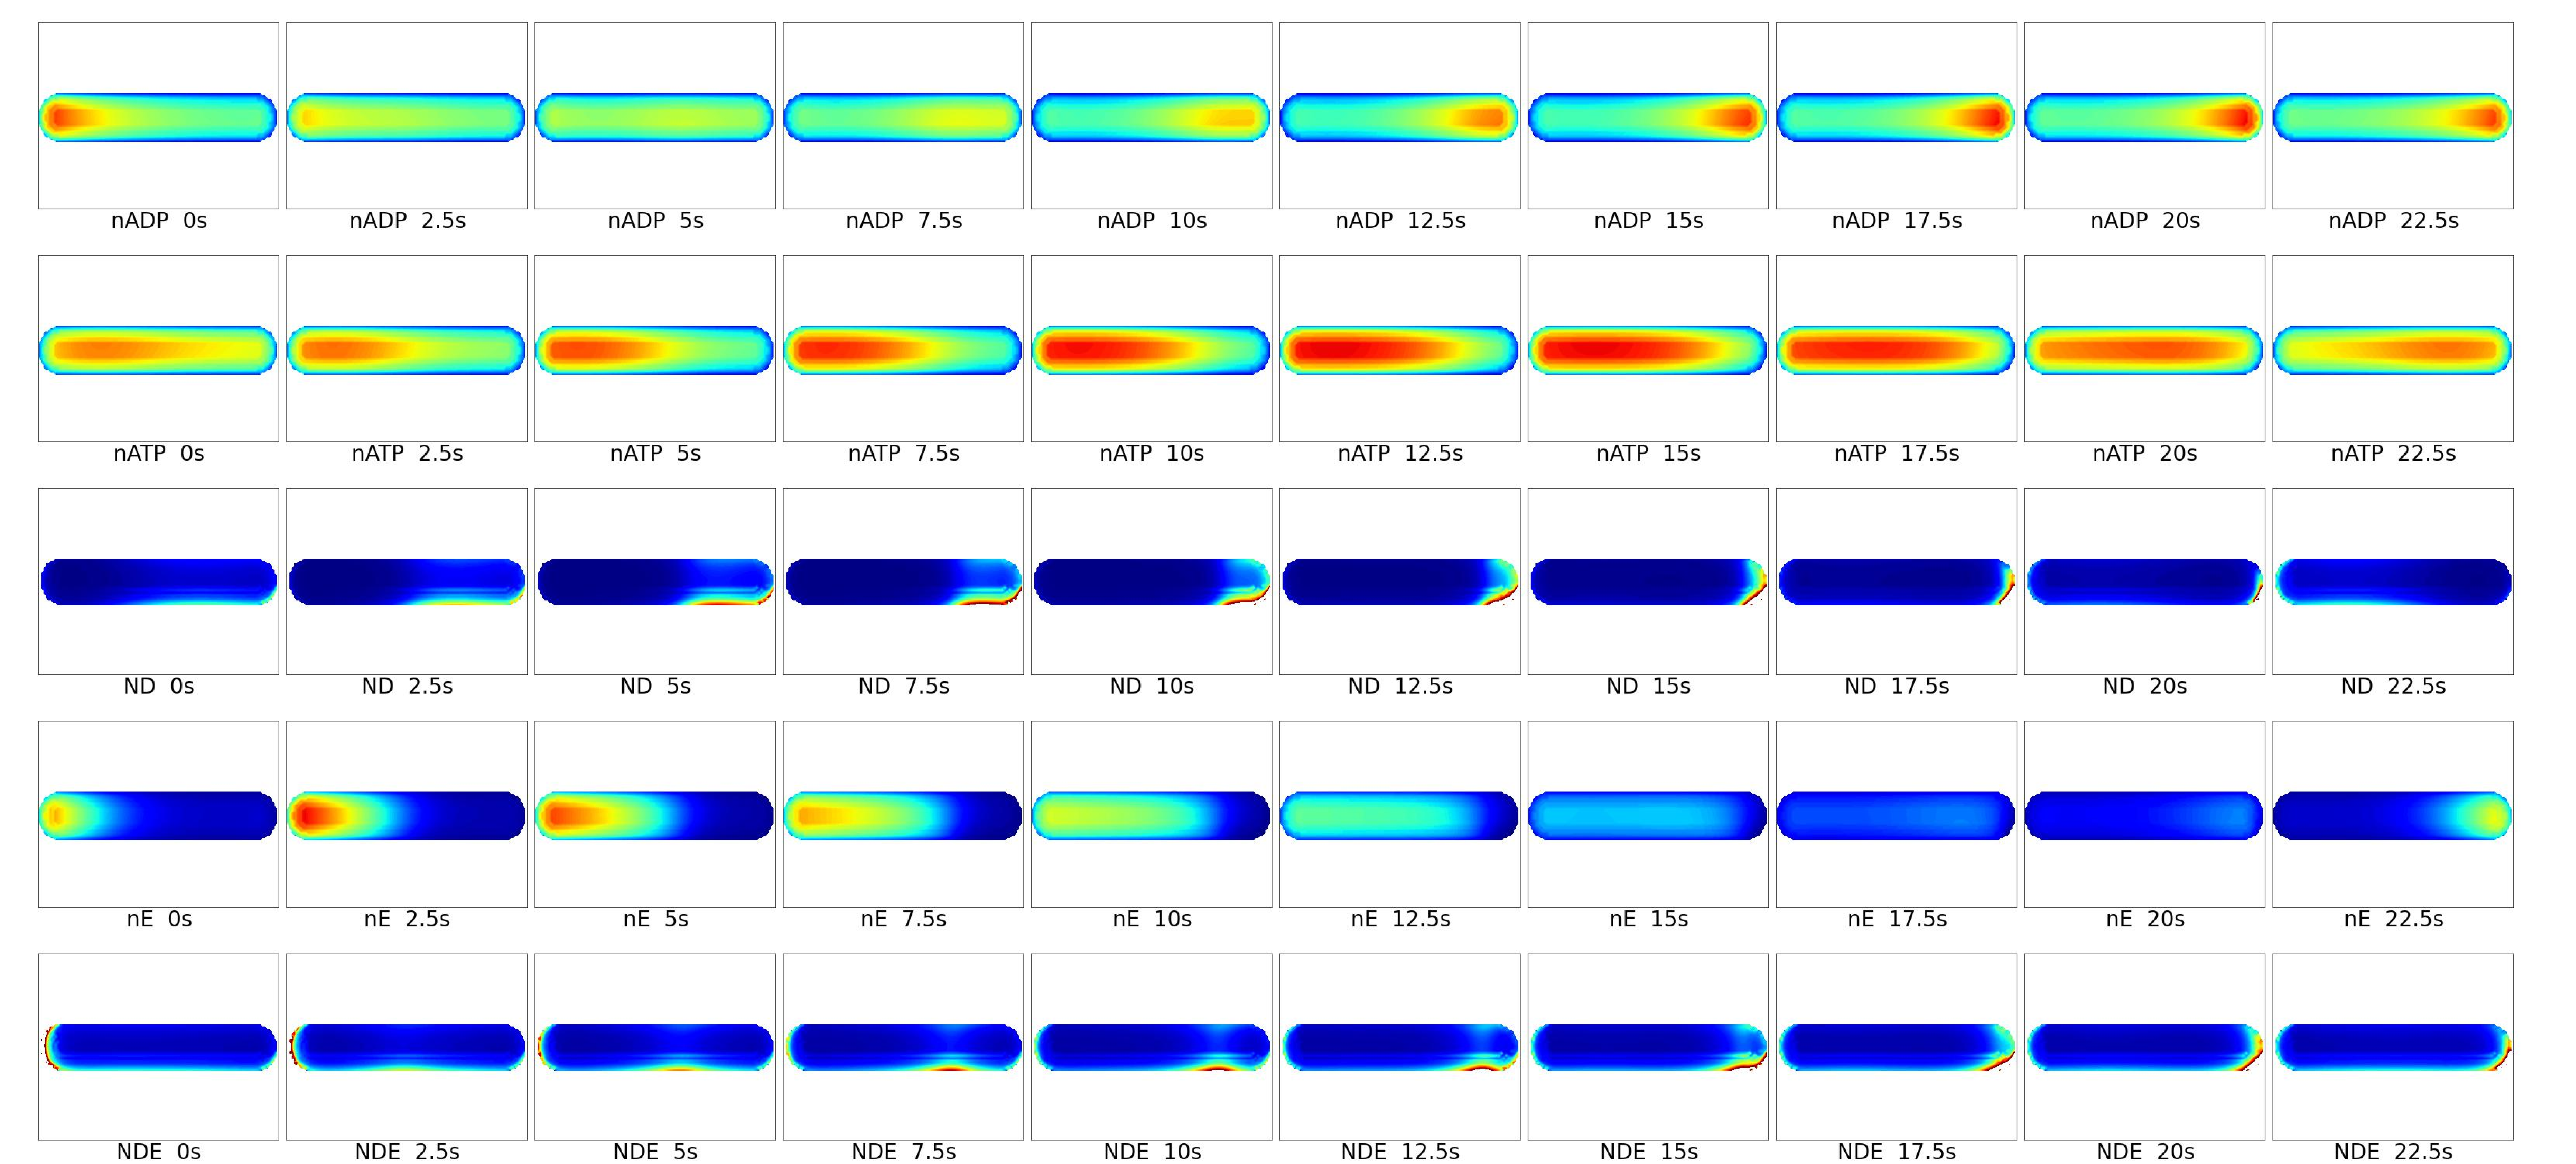
\includegraphics[width=\textwidth]{../data/shape-p/plots/image-plot--p-400-50-0-0-1500.pdf}
  \caption{Frames from an animation showing a series of contour plots
    of the concentration of proteins in different stages over time.
    The density of proteins are integrated along the axis
    normal to the page. The frames occur 2.5 seconds apart.}
  \label{image-p}
\end{figure*}

Consider Figure \ref{image-p}.  At 0 seconds we can see cytoplasmic
nATP roughly evenly distributed throughout the cell.  There is nADP
concentrated in the left pole and it will transform into nATP.  At 2.5
seconds we see membrane bound MinD:ATP form on the right side of the
cell.  It avoids the left side because there is a concentration of
cytoplasmic MinE on the left side and compared to the right side,
which is empty of MinE, MinD:ATP attaching to the wall on the left has
no time to collect and cluster before reacting.  One can see how as
the MinE spreads out rightward, the the clustered membrane bound
MinD:ATP stays just at the edge of it, always to the right.  Where the
two meet there is at every time step a spike in membrane bound
MinD-MinE:ATP, resulting from the MinE reaction with the MinD on the
wall.  One can see from roughly 5 seconds to 17.5 seconds the
cytoplasmic MinE chases in a way the MinD towards the right, reacting
with it as it clusters on the wall.  Upon reaching the right side, the
MinD is in a way trapped, and the MinE now concentrated in that pole
will react until the MinD has diffused back towards the other side and
there is no more membrane bound MinD:ATP to react with.  The cycle
then begins again.



\begin{figure}
  %%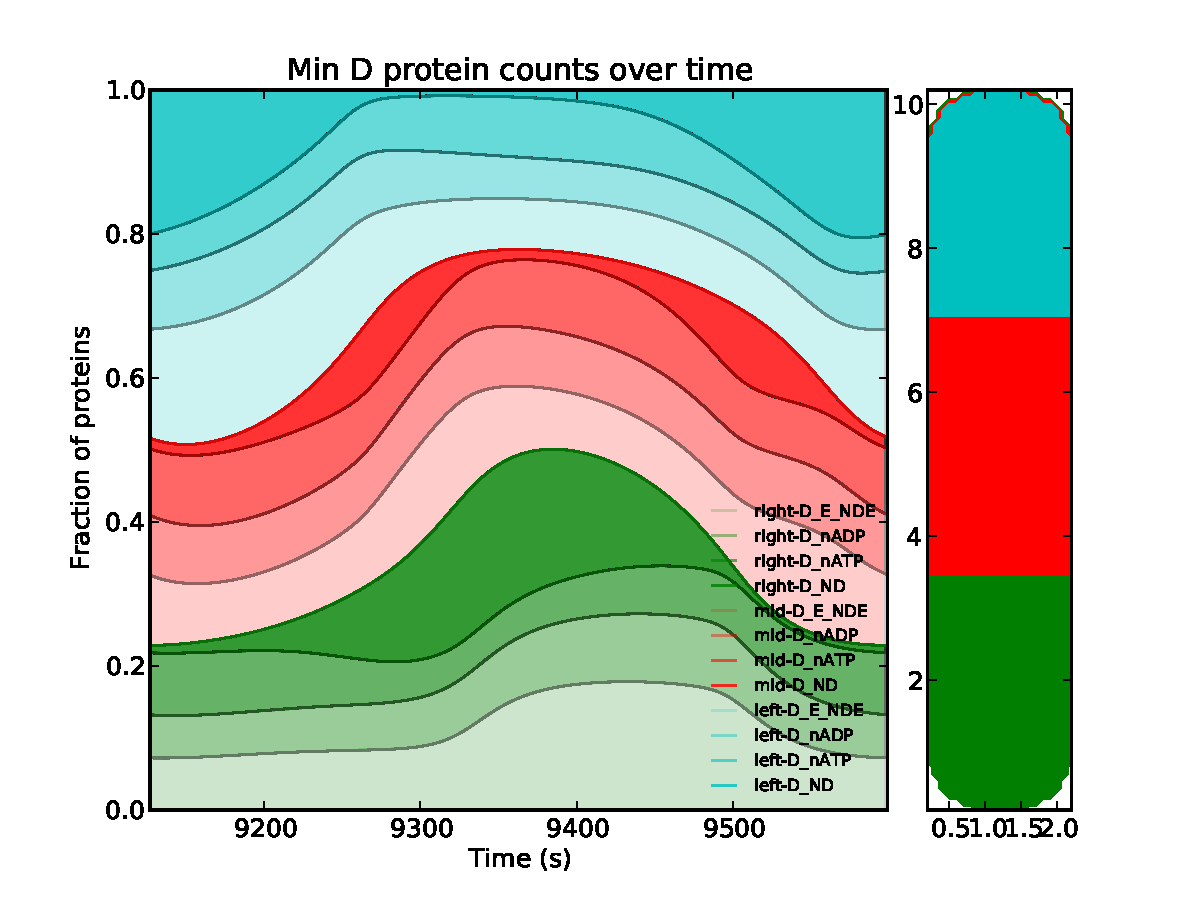
\includegraphics[width=\columnwidth]{../data/shape-p/plots/box-plot_D--p-400-50-0-0-1500}
  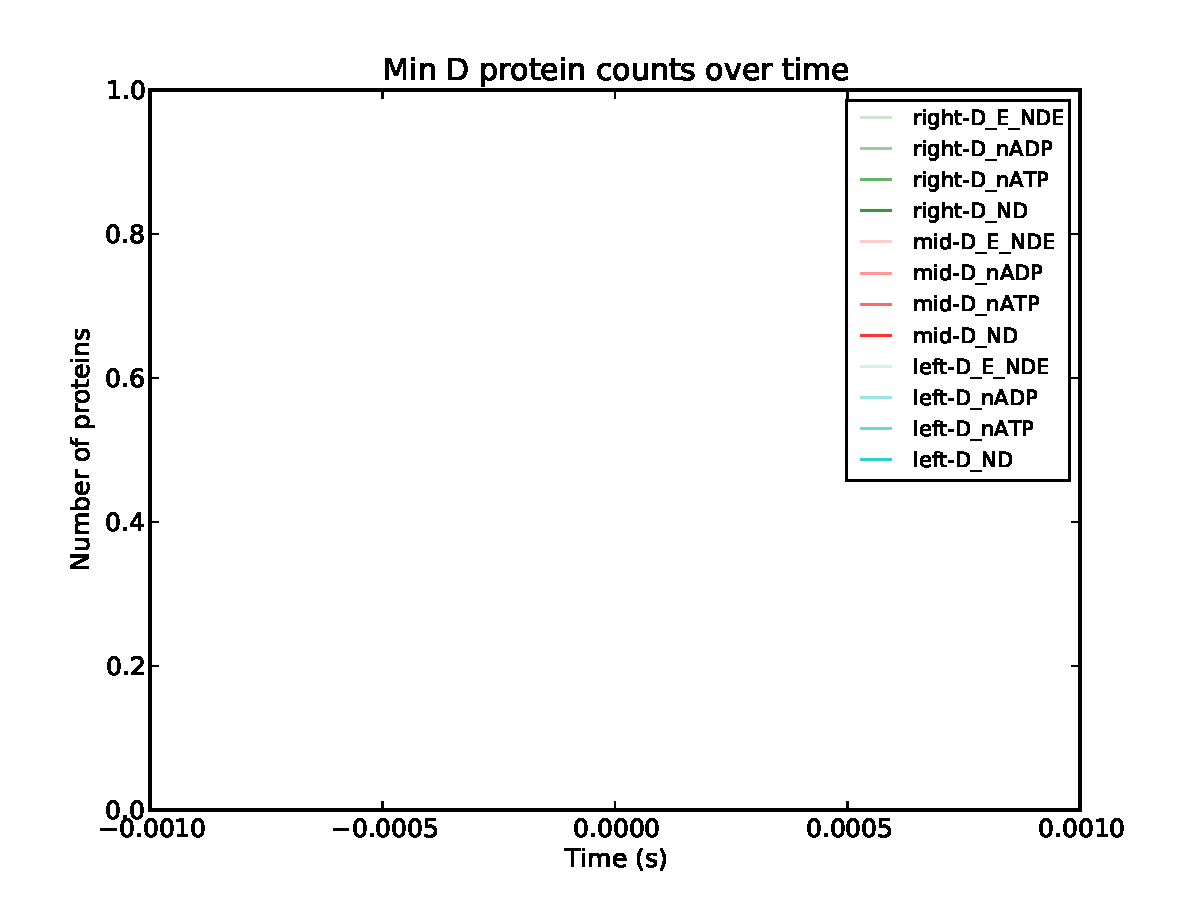
\includegraphics[width=\columnwidth]{../data/shape-p/plots/box-plot_D--p-200-50-0-0-1500}
  \caption{Total protein fluctuation in the right, middle, and left
    parts of a 5$\mu m$ by 1$\mu m$ pill shaped cell (above) and a
    3$\mu m$ by 1$\mu m$ pill shaped cell (below).  The vertical axis shows
    stacked the total number of proteins that are of four different
    compound stages and in the right section of the cell (bottom four
    colors), in the middle of the cell (middle four colors) and in the
    left section of the cell (top four colors). The different forms of
    protein changes while the total number of MinD protein in the cell
    remains constant, shown by the fact that the very top line is
    horizontal.}
  \label{box-p}
\end{figure}

Figure \ref{box-p} is a plot of the total fraction of
MinD found in each stage of the cycle in each of three sections of the
cell (we have split the pill into two polar sections and one center
section) over time.  One complete oscillation period is shown, in
which one of the poles begins and ends at a maximum density
concentration and the other a minimum density concentration.  Looking
at the evolution of the latter, we see an initial high concentration
of cytoplasmic MinD:ATP, as the this protein diffuses into the polar
region, followed by a dip in this and large spike in membrane bound
MinD:ATP, as the protein clusters onto the polar cell wall, followed
by a spike in the memebrane bound MinE:MinD:ATP stage of protein,
together with a slight rise in cytoplasmic MinD:ADP as the MinD
dettaches from the wall.

results for pill shaped cell of length
$5\mu$ and radius $.5\mu$.  The plot shows both the transerence
between different stages of protein compound and movement within the
cell.  Starting at the beginning of a period, we can see that first
there is a spike on the left of MinD-ATP attached to the wall that is
accompanied by a growing number of cytoplasmic MinD-ATP and MinD-ADP
that are entering the left section, followed by a high peak in
MinD-MinE-ATP.  This peak gives way through the middle to peaks on the
right side of the cell, the first being a small bump in cytoplasmic
MinD-ATP that dissapears into a much larger spike in wall attached
MinD-ATP, which is followed by a peak in wall attached MinD-MinE-ATP.
The pattern during each period clearly shows the cycle of proteins
rections, as well as the very regular nature of the pole to pole
protein oscillations.

\fixme{our 5 length cells are labeled as 4 cells in the file labels,
  since 4 is the length of the cylinder. In the text I'll refer to the
  5 length cells (file says 4) as 5 length cells.  What huang's paper
  calls 4 length cells will be labeled by our files as 3 length cells,
  but will be refered in our text as 4 length cells}.  We can see a
clear difference in period between the $5\mu$, $4\mu$, and $2\mu$
length cells.  The oscillation periods for our $4\mu$ show excellent
agreement with the simulations of Huang et all
\cite{huang2003dynamic}.  This is to be expected since we begin our
simulations with their reported wild type concentrations of MinD and
MinE proteins. The periods for the different pill lengths are shown in
the table below.  We can see a direct correltation between size and
period, as the proteins must diffuse further in a longer cell before
they accumulate on the opposite wall.

\begin{table}
  \begin{tabular}{|r|c|c|c|l|}
    \hline
    Length($\mu$) & 2.50 & 3.00 & 4.00 & 5.00\\
    \hline
    Period(sec) & sim & 33 & 38 & 48 \\ \cline{2-2}
    \hline
  \end{tabular}
  \caption{Period According to Pill Length}
\end{table}

\begin{figure}
  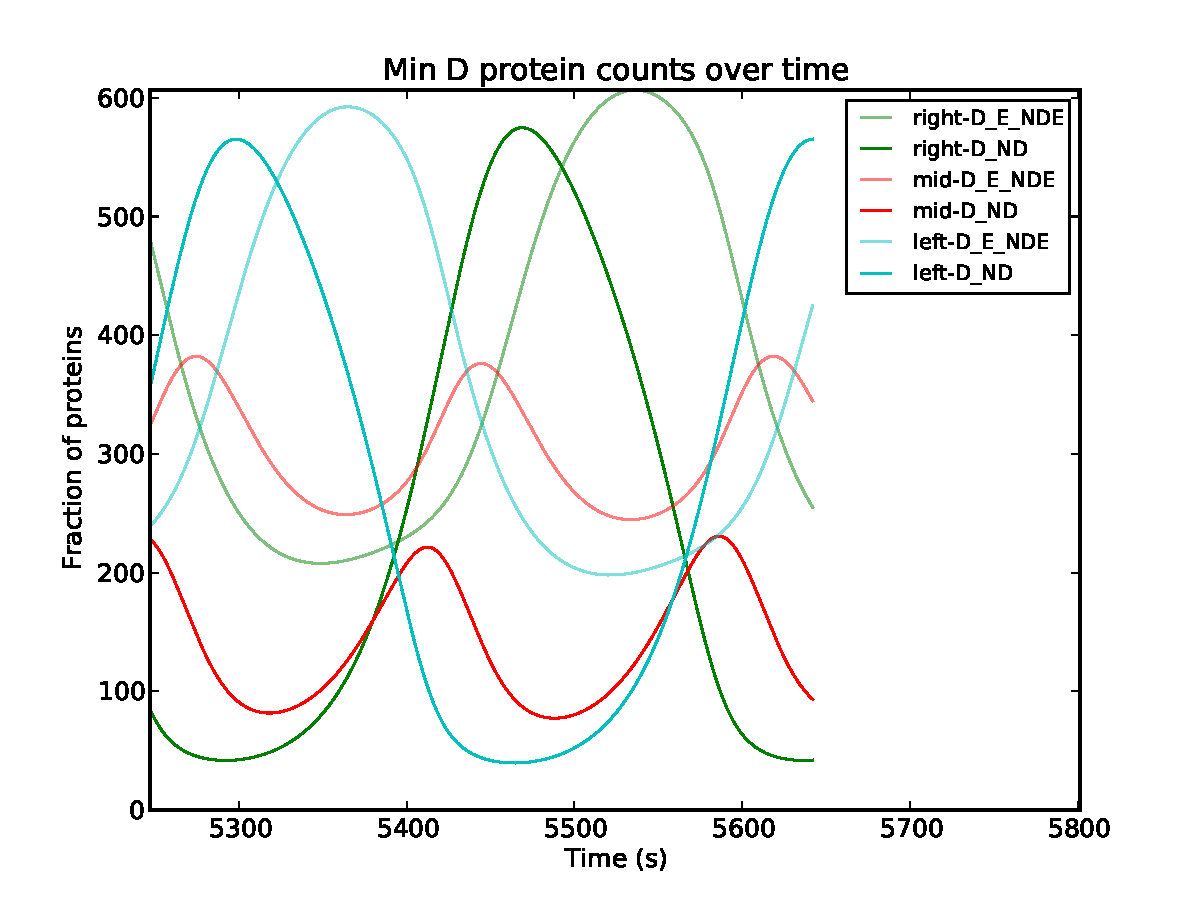
\includegraphics[width=\columnwidth]{../data/shape-p/plots/ave-plot_D--p-200-50-0-0-1500}
  \caption{Average protein density per unit area of wall for the wall
    attached stages of the protein cycle.  Shown in the right, middle,
    and left parts of a 5$\mu m$ by 1$\mu m$ pill shaped cell (above)
    and a 3$\mu m$ by 1$\mu m$ pill shaped cell (below).}
  \label{ave-per-area-plot-pill}
\end{figure}

Figure \ref{ave-per-area-plot-pill} shows the ave protein per unit
area that is wall attached in the middle, right, and left sections of
the pill shaped cell.  This is an important test of the central idea
behind the utility of the Min protein system.  The system is meant to
place Min proteins on the walls in heavier concentrations in the caps
of the cell and lower concentrations in the middle section, so that
the FtZ polymer may build up along the center walls.  We can see from
the plot of the 3$\mu m$ by 1$\mu m$ cell that the MinD proteins reach
concentration peaks in the caps that are higher than peaks in the
center.  \fixme{is the next part true?} Integrals of these plotted values show that the time averaged
concentrations are likewise higher in the caps than in the center.

\subsection{Triangular Shapes}
\begin{figure}
  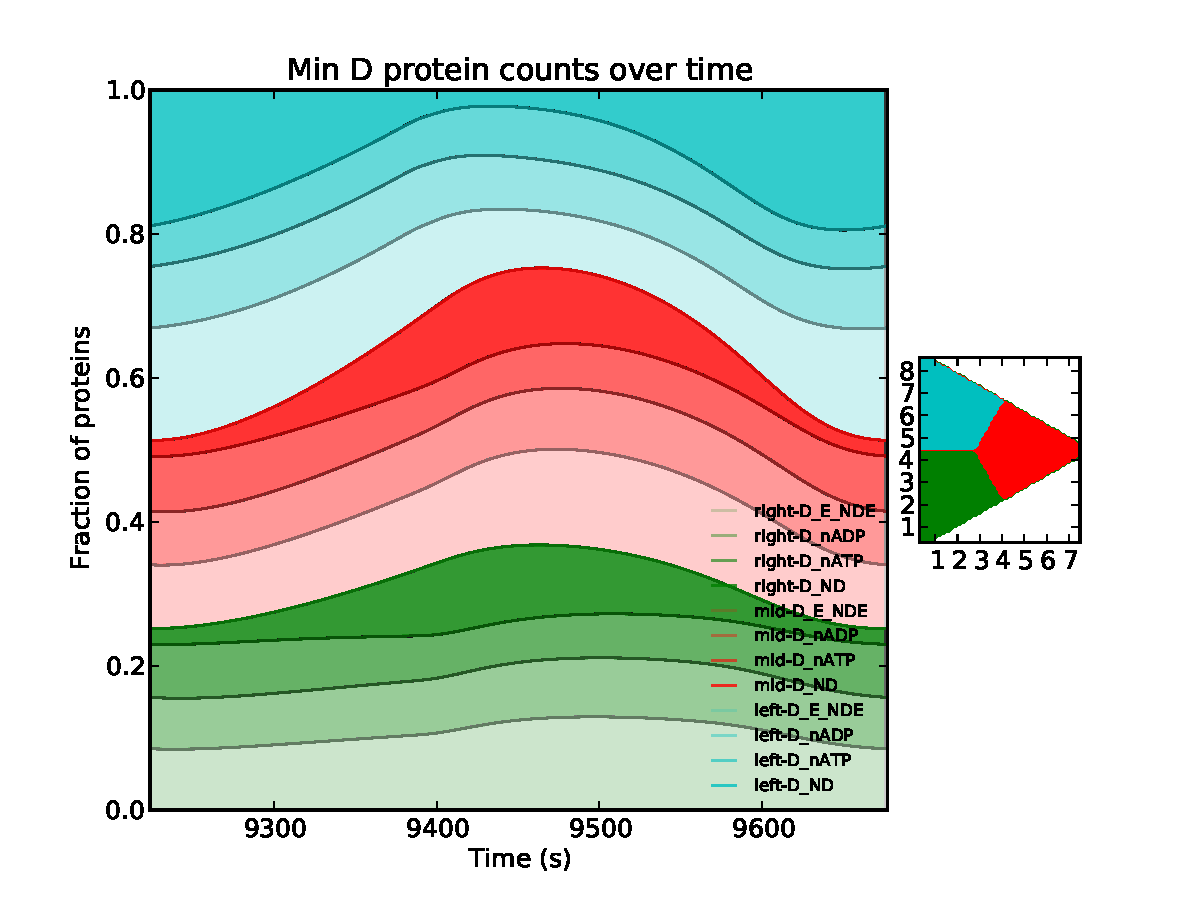
\includegraphics[width=\columnwidth]{../data/shape-triangle/plots/box-plot_D--triangle-25-400-400-400-1500}
  \includegraphics[width=\columnwidth]{../data/shape-triangle/plots/box-plot_D--triangle-25-500-300-500-1500}
  \includegraphics[width=\columnwidth]{../data/shape-triangle/plots/box-plot_D--triangle-25-600-480-360-1500}
  \caption{Total protein fluctuation in the right, middle, and left
    parts of a equilateral (top), iscoscolese (middle), and 3-4-5
    (bottom) triangle.  The vertical axis shows stacked the total
    number of proteins that are of four different compound stages and
    in the different sections of the cell.}
  \label{box-triangle}
\end{figure}

The double pole oscillation pattern, where one pole is located in a
single corner of the triangle and the other pole is spread out between
the opposite two, can be seen in Figure \ref{box-triangle}.  The
equilateral triangle shows a spike in both the Center and Left
sections at the same time, both showing the familiar sequence of peaks
amoungst the different states of the protein seen in the poles of the
pill shaped bacteria.  A spike in the other corner, showing the common
sequence, occurs during the minima of the former two, wth a higher
concentration at the peak.  A similar pattern is seen in the
iscosolese triangular shape, where interestingly the onset of the
maxima in the single maxima corner (the Left section) builds more
quickly than it fades.  This is presumably becuase as the cytoplasmic
minD:ATP diffuses down a more accute corner, it is sourrounded by
closer cell walls than it would be in a less acute corner, so that the
it is more apt at any diffusive step to make contact and cluster on
the walls.  That particular part of the process is therefore
accelerated, driving the build up of the maxima forward.  The right
triangle shows a similar pattern.



Figure \ref{total-oscillation-triangle-plot} shows the equivalent
motion and transference between compound states for the triangular
states as Figure \ref{total-oscillation-plot} does for the pill shaped
cells.  The equilateral triangular shows that in all three sections
there is a spike in wall attached MinD-ATP directly followed by a
spike in wall attached MinD-MinE-ATP.  The pill had shown a similar
pattern except that the mid section exhibited no such pronounced
spike.  Interestingly, the right and mid sections show spikes at
similar times when compared to the left section spikes, which seem to
oscillate in a manner shifted pi off from the other two.  This
behavoir shows itself in the animations, which show a relaxation into
a stable oscillation from a maxima in one corner to a double maxima in
the other two corners, and back again.  The left section heights are
roughly twice that of the right section heights.  The simulations are
started with higher concentrations of proteins in primarily the right
section, with some overlap into the middle section, so that perhpas
this oscillation pattern seems reasonable.  However, it's interesting
to note that the oscillations, started with assymmetric density, do
not naturally rotate around the corners of the triangle in a circular
pattern.


It seems as well that there is a desired oscillation maxima for the
particular shape and size of the cell, as can be seen by the
relaxation, over the first four periods, to a regular maximal height
of the right and left sections' total protein at the height of each spike.

\fixme{Note to make sure I'm interpreting the iscosolese triangle data
  correctly: the triangle sides are 5,5,3, and the higher density
  starts in the corner that is opposite the short side.  This corner
  is covered by the right section.  I've verified this by looking at
  the protein\_microscopy and drawing a little picture, which is on my
  desk...if you dare look for something on my desk!!!}  The iscosolese
triangle starts its simulation with a higher concentration of protein
in the section that is opposite the shorter side.  It quickly relaxes
into a stable oscillation pattern.  This pattern shows that right
corner section regularly has higher spikes in total protein than the
other sections, and that its spikes appear one pi removed from the
spikes for the other two sections.  This a similar behavoir to that
which is seen in the equilateral triangle, differening in that it
converges more quickly towards this behavoir and that it shows a
greater exageration in the height of protein buildup in the right most
section.

\fixme{Note on interpretation of 3-4-5 triangle: the higher density
  starts to the right of a vertical line that is parrallel to the
  second longest side in the triangle (the longer of the two
  non-hypotonuse sides).  This means the higher concentration covers
  the right angle and also the smaller angle in the triangle} The
3-4-5 triangle exhibits behavoir that I need more data to properly
observe.  I does not converge as quickly as that for the iscosolese or
equilateral triangles.

\subsection{Randst shape}
\fixme{Cheat sheet for the shapes, need to put these into a big figure
  from the sections output: 96=star shape, 97=sideways sideways
  flying saucer pancake, 98=manniks squished cell, 99=an A}

\subsubsection{Randst-mannik shape}
\begin{figure}
  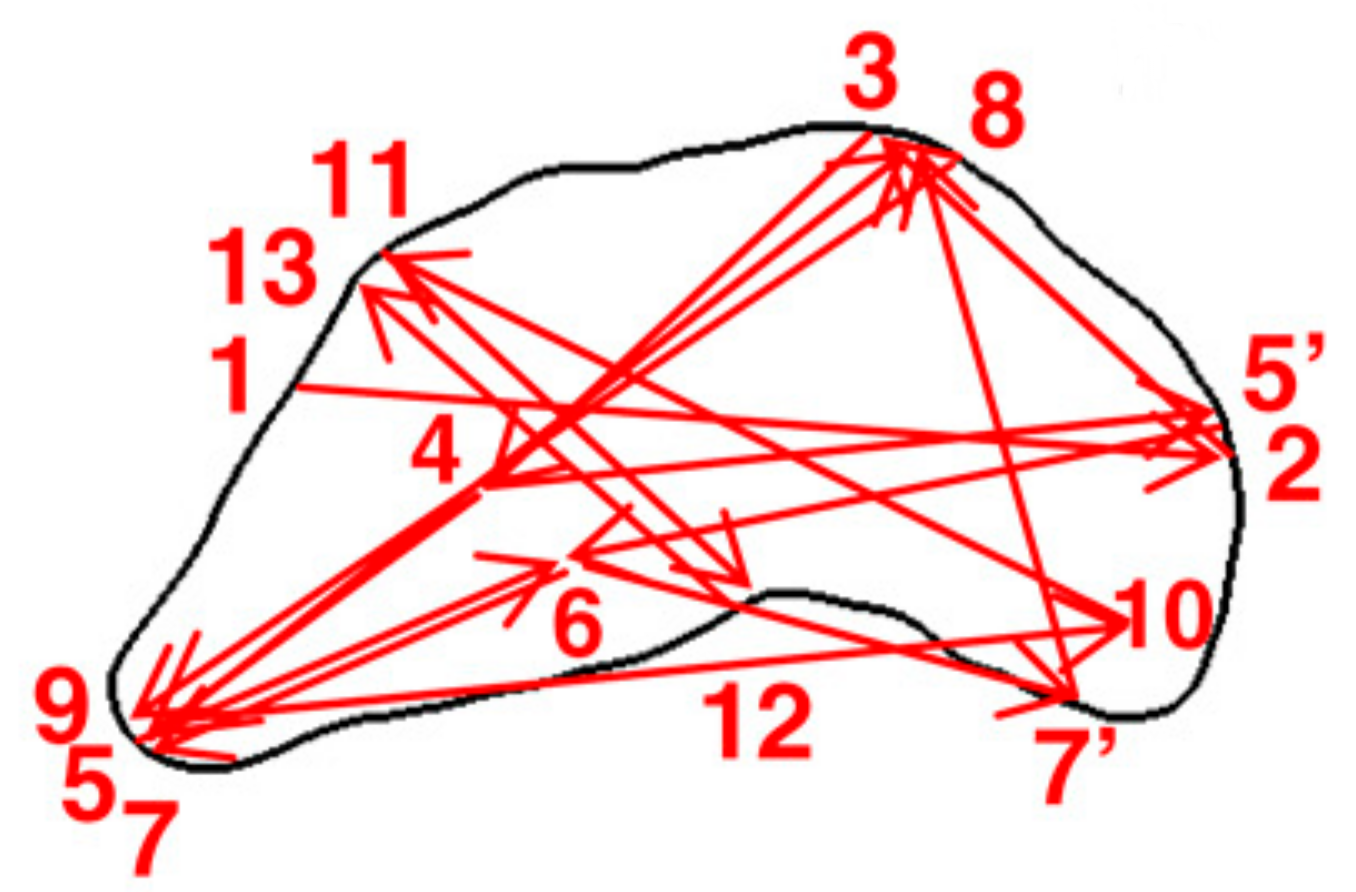
\includegraphics[width=2.8cm]{../mannik-2.png}
  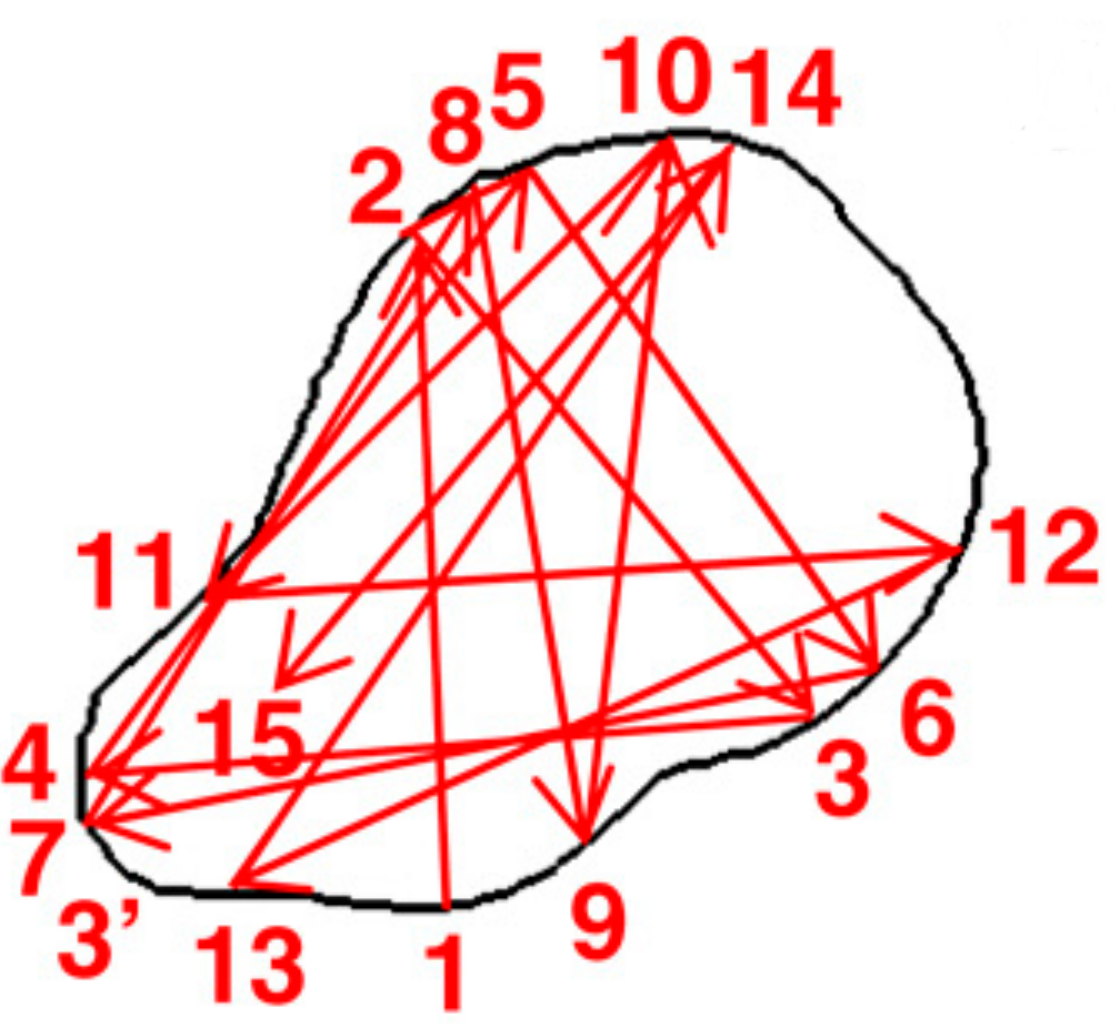
\includegraphics[width=2.8cm]{../mannik-1.png}
  \includegraphics[width=3cm]{../data/shape-randst/plots/arrow-plot-NflD-randst-25-1300-2000-9400-1500.pdf}
  \includegraphics[width=3cm]{../data/shape-randst/plots/arrow-plot-NflD-randst-25-1101-1101-9500-1500.pdf}
  \includegraphics[width=3cm]{../data/shape-randst/plots/arrow-plot-NflD-randst-25-600-800-9800-1500}
  \includegraphics[width=3cm]{../data/shape-randst/plots/arrow-plot-NflD-randst-25-1102-1102-9500-1500}
  \caption{Arrow plots for our simulation and mannik's experimental}
  \label{arrow-compare-mannik}
\end{figure}

Figure \ref{arrow-compare-mannik} shows a comparison of time maxima
plots with similar plots published by mannik et al.  The sequence of
arrows show a series of global maxima in space and local maxima in
time at their heads, numbered by the sequence in which they occur.
They function as a trace of the path that the traveling maxima take.
We have created for each of the two shapes published by Mannik a
closely resembling shape (shown directly below Mannik's) and a
variation on this shape (shown below that) in order to test the effect
of variations on basic shapes.  The plots of the left shape show that
much of the preffered locations for the proteins to maximize are
similar between this experimental and simulated shape.  The maxima in
the top center of the cell does not seem to appear in the experimental
version.  Also in both of the simulations on the left there don't seem
to be maxima at membrane regions with negative radii of curvature
while the experimental shows a maxima in the bottom center region
right at one of these regions.  The shape on the right compares less
successfully.  Here the simulation shows a limited number of maxima
locations that appear to be quite regular, where mannik's experimental
results show a much more chaotic system.  In particular, the maxima
location on the right wall seems to be very robust.  It acts as one of
the poles do in the pill shapes.  \fixme{I'm now running a sim with a
  slightly different shape to see result} The simulated version has
found a robust two pole pattern, similar to that seen in other shapes.





\subsubsection{Randst-99 our lambda shape}
\begin{figure}
  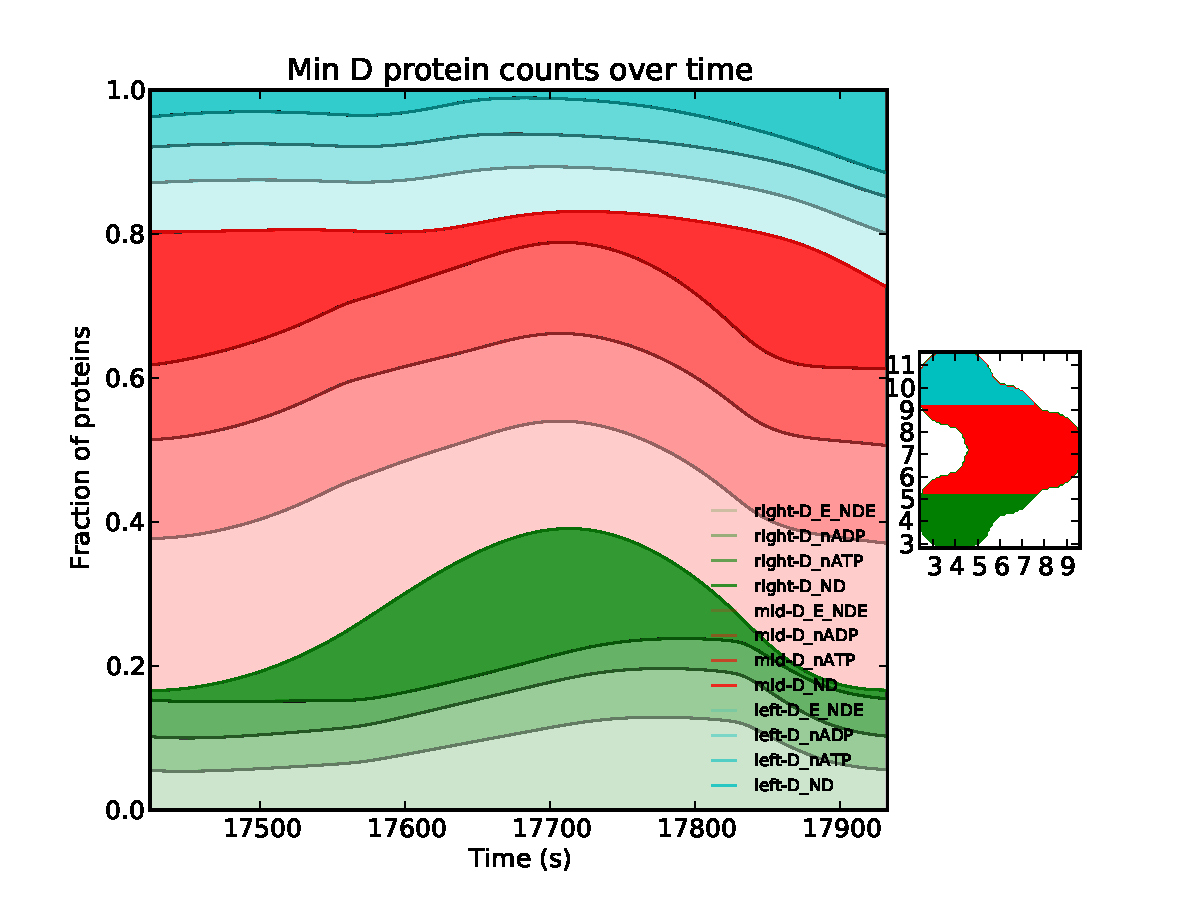
\includegraphics[width=\columnwidth]{../data/shape-randst/plots/box-plot_D--randst-25-600-600-9900-1500}
  %%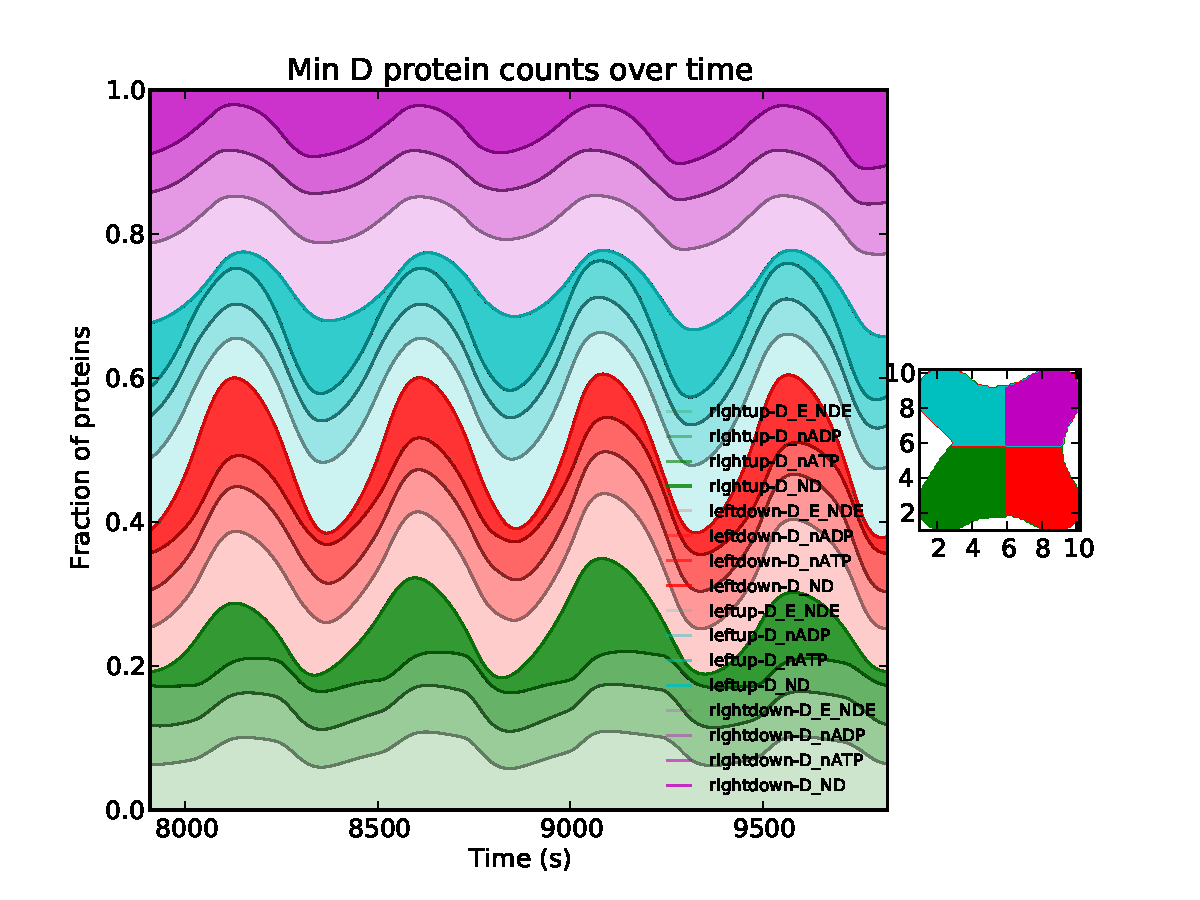
\includegraphics[width=\columnwidth]{../data/shape-randst/plots/box-plot_D--randst-25-600-600-9600-1500}arrow-plot-NflD-randst-25-600-800-9800-1500.pdf

  \caption{Total protein fluctuation in the A shaped shape.  The vertical axis shows stacked the total number
    of proteins that are of four different compound stages and in the
    different sections of the cell.}
  \label{total-oscillation-randst-96-plot}
\end{figure}



Our animations for this cell shape show a very interesting pattern.
The maxima oscillates from the right corner to the top corner, then
\emph{back to the right corner} then to the top corner again, then to
the left corner, then back to the top, then to the left, then to the
top again, then back to the right side.

\fixme{running larger and smaller.  Guessing the larger will do pole
  and pole, so talk about in terms of you have huge, pole and pole,
  then once get small enough double oscillations develop.  Why do they
  do that?  And hen you can do image plot for the one with consistent
  double oscillations.  Can right now explain reason for double
  oscillations.  Look at todo.txt.  The slightly varied guassian shape,
  so a little assymetric, doesn't change double oscillation pattern.}

Contour plot frames from the animations show the second maxima in the
lower left corner (immediately following the one in the upper middle
corner) will reside for a bit longer than the left corner maxima
preceding it.  These longer residing maxima will then be followed by a
switch, to the right corner, with a short, less intensive maxima
traveling through the center.  The MinE shows the same pattern. The
MinE that was just concentrated on the left corner during the first
maxima, after releasing the MinD from the membrane there, diffuses up
and attaches to the MinD on the upper corner membrane and begins to
release it.  During this process the MinE starts at the edges and
moves in towards the center of the maxima.  The center of the cup is a
little further away so it attaches to these outer ridges first and
then moves in.  After it eats at the corners and starts moving in the
MinD eventually travels back to set up a maxima in the left corner.
Watching the cytoplasmic MinE, something very interesting: It as well
maximizes twice in the left corner, but during the MinD's first maxima
in the left corner, the MinD has a maxima in the upper corner, and
during the MinD's second left maxima, the MinE travels to the right
corner and has a maxima there.  At the same time (during the second
MinD left corner maxima), there is a large amount of cytoplasmic
MinD:ATP on the right side.  The MinE does this becuase during the
first MinD left corner maxima, the MinE has just come off a maxima in
the right corner.  So it diffuses up to the upper corner and sets up
there.  During the second MinD left corner maxima, the MinE has just
come off the upper corner maxima.  It will diffuse into the right
corner and left corner.  In the left corner it interacts with the MinD
bound to the membrane there.  In the right corner it sits and
eventually diffuses away, but at a somewhat slow pace.  \fixme{An idea
  is that once the MinD travels back from the left corner after its
  second maxima there, it is not able tot set up a maxima in the upper
  corner as easily, since there is left over MinE there, which has
  just traveled from the right corner.  The problem with this is that
  the MinE doesn't seem to be maximized in the upper corner when the
  MinD is traveling back up from the left.}  The other idea is simply
that because the minE is traveling all the way from the right corner,
the longer time it takes to get there simply means that it all
concentrates on the left, leaving the upp and right side completely
open for the build up of MinD.  \fixme{Still dont quite get it but
  take a look at the other simulations and come back.} Actually, you
can see this effect very slightly watching the 98 shape, between the
center cap and the right corner.




%% \begin{center}
%%   \begin{figure}
%%     {\includegraphics[width=\paperwidth]{../data/shape-randst/plots/image-plot_E--randst-25-602-602-9900-1500}}
%%     \caption{Attempt at adding image plot to paper.}
%%     \label{image-plot}
%%   \end{figure}
%% \end{center}
\subsubsection{Randst-96-Star}
\begin{figure}
  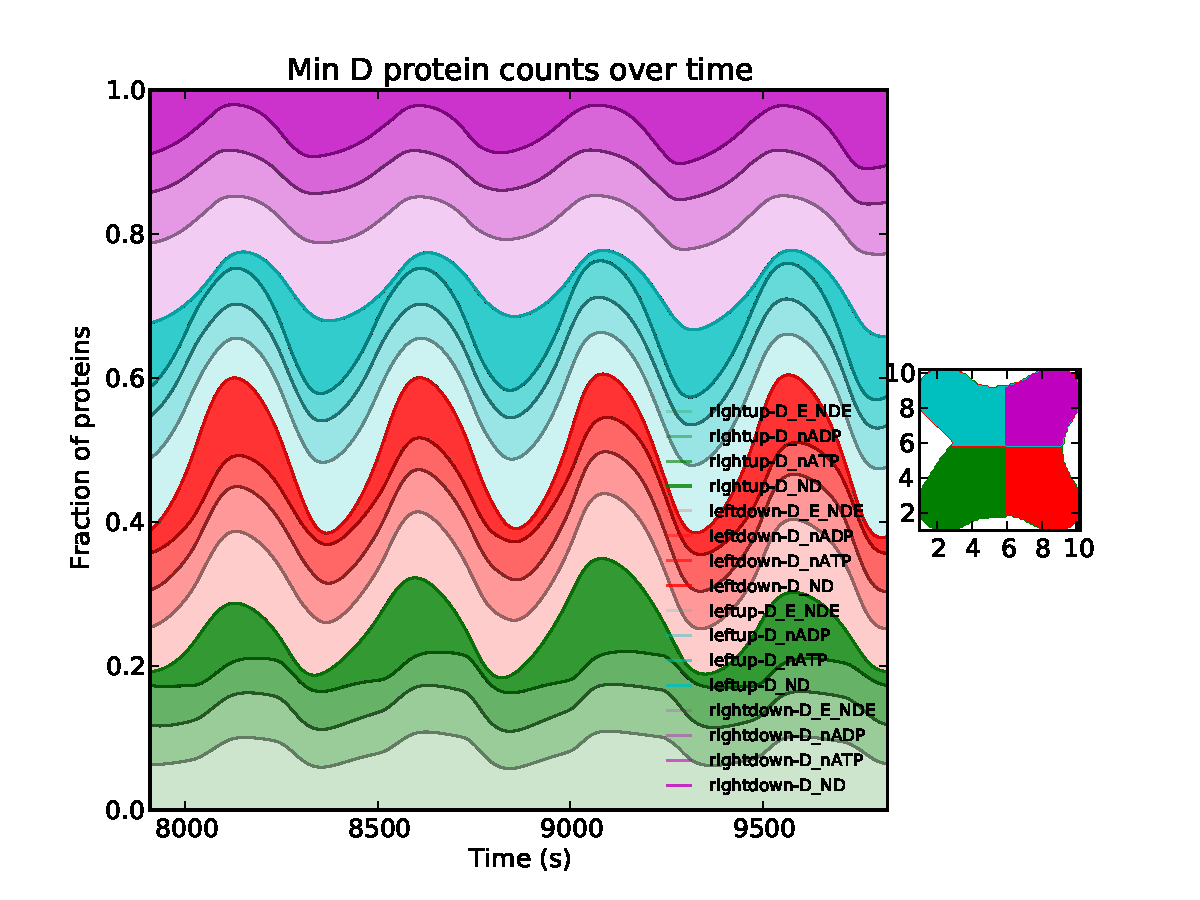
\includegraphics[width=\columnwidth]{../data/shape-randst/plots/box-plot_D--randst-25-600-600-9600-1500}
  %%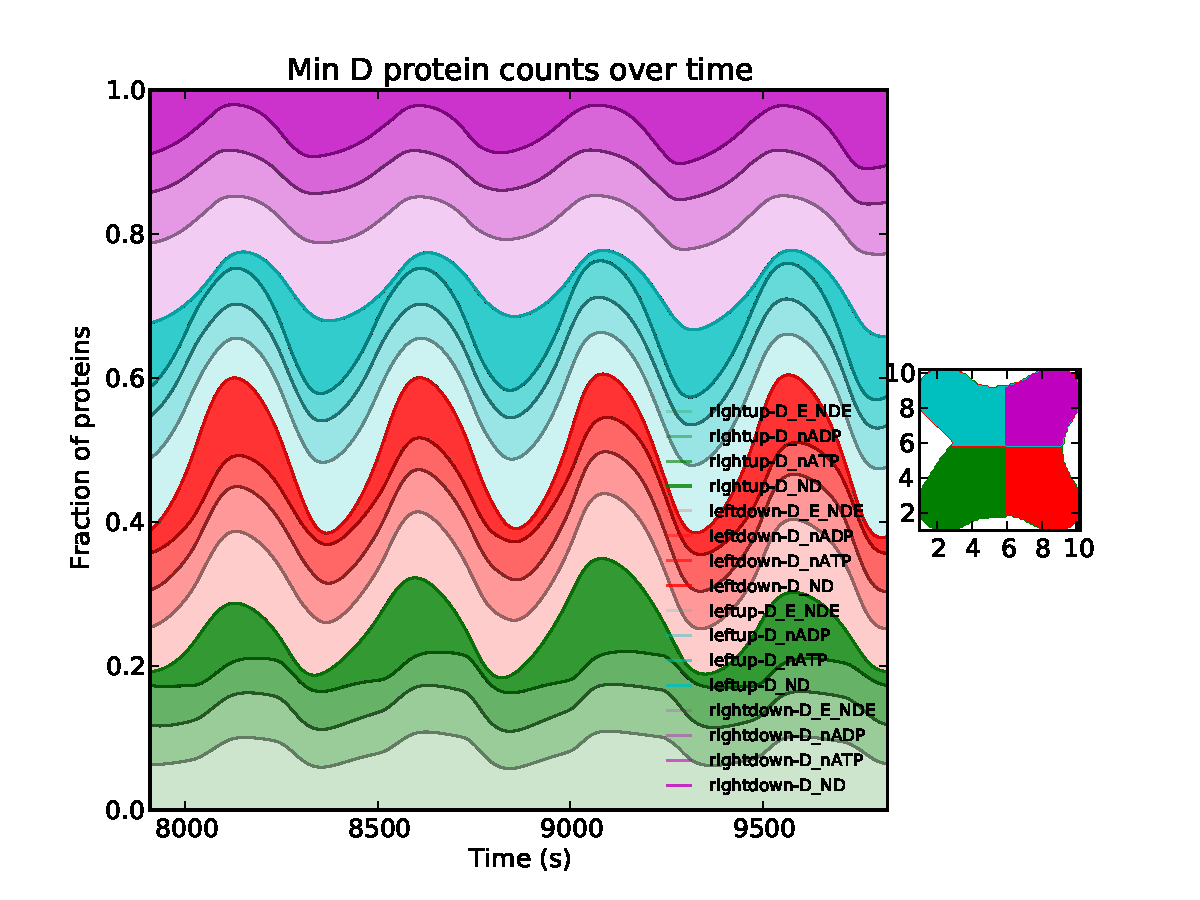
\includegraphics[width=\columnwidth]{../data/shape-randst/plots/box-plot_D--randst-25-600-600-9600-1500}
  \caption{Total protein fluctuation in the star cell shape.  The vertical axis shows stacked the total
    number of proteins that are of four different compound stages and
    in the different sections of the cell.}
  \label{total-oscillation-randst-96-plot}
\end{figure}

Looking at at few periods in detail.  We find that there is a small
increase in cytoplasmic MinE always directly before the the beggining
of climb in the membrane bound MinE peak.  Also, there is at any one
time a very large amount more of minE that is membrane bound then
cytoplasmic in any ones section.  A difference of a factor of roughly
20 when membrane MinE is at its peak, and roughly 12 when membrane
MinE is at it's minimum.  There seem to be two modes of oscillation,
each exhibiting a density peak maxima that moves back and forth
diagonaly from one corner to the opposite, as if there were two
overlapping, criss-crossed cells oscillating.  In the box plot this is
seen as roughly coinciding membrane minD peaks in the lower left and
right corners, followed one pi later in peaks in the upper right and
upper left corners.  Interesting that this did not exhibit
counterclockwise motion that Huangs 2008 paper might suggest.  Should
run sims that start in the wacky way that just started running with
triangles.
\newline


We haven't simulated long enough yet, so no real pattern has shown
itself.  There's certainly oscillations, and it's almost as if there's
competing modes - top to bottom, left to right, corner to corner, etc.
Interesting.

\fixme{maybe?}The animations seem to relax into a pattern in which the oscillations
go from the smallest corner, out to the other three, and then back to
the smallest corner?  \fixme{There isn't enough data to see properly
  though, need to run for longer.}

\subsubsection{Randst-97-}
\begin{figure}
  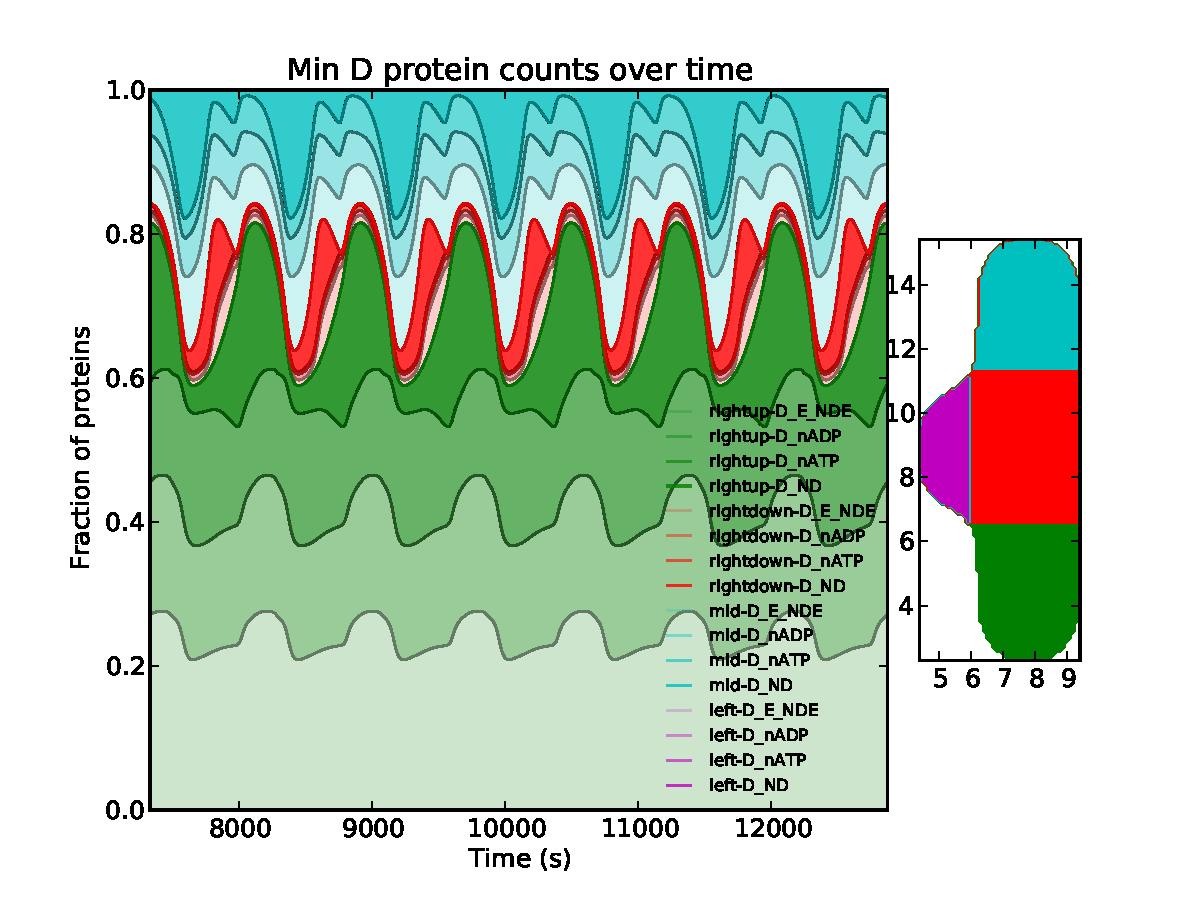
\includegraphics[width=\columnwidth]{../data/shape-randst/plots/box-plot_D--randst-25-800-600-9700-1500}
  %%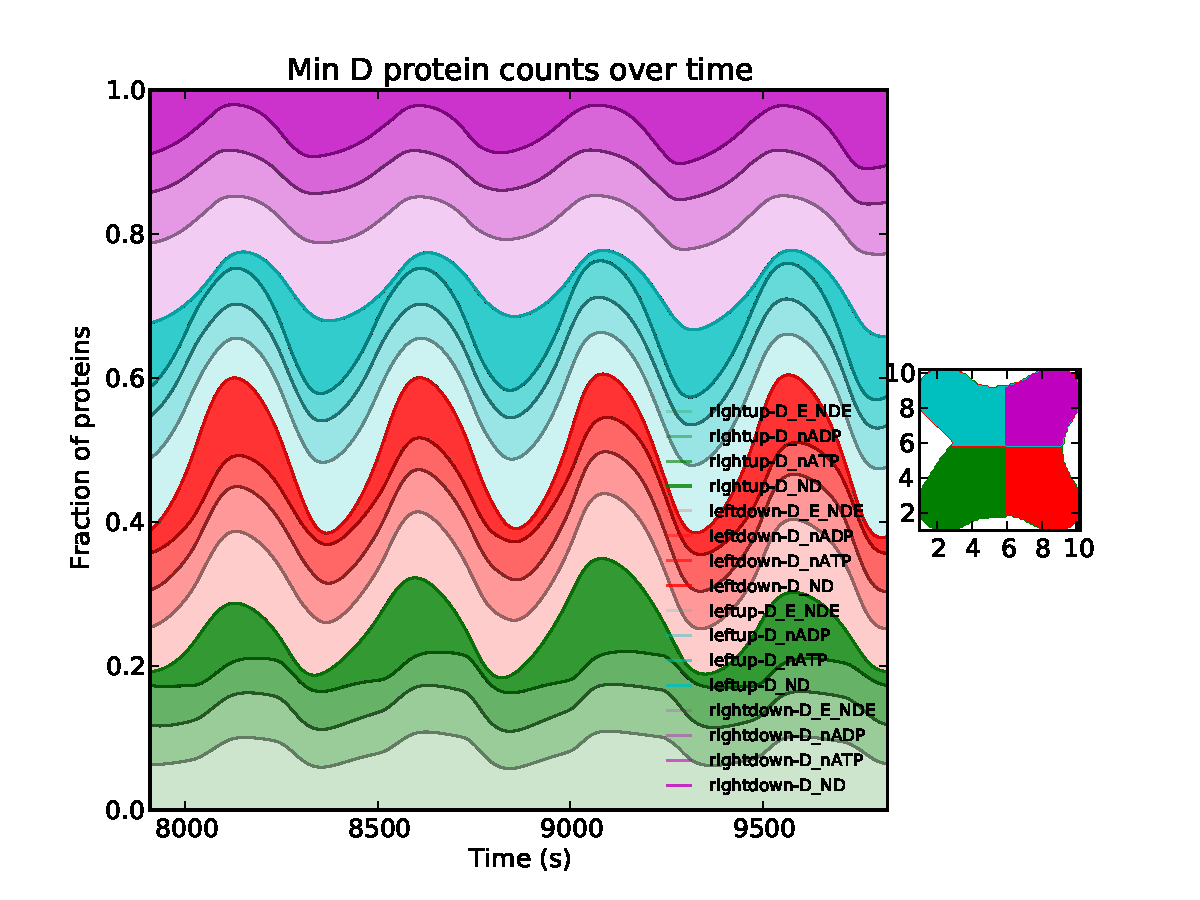
\includegraphics[width=\columnwidth]{../data/shape-randst/plots/box-plot_D--randst-25-600-600-9600-1500}
  \caption{Total protein fluctuation in the sideways flying saucer
    pancake cell shape.  The vertical axis shows stacked the total
    number of proteins that are of four different compound stages and
    in the different sections of the cell.}
  \label{total-oscillation-randst-97-plot}
\end{figure}

The sideways flying saucer pancake shape shows a truly interesting
breakdown of an unstable equilibrium oscillation.  For the first
number of oscillations the maxima trade off right to left, from a high
peak in the leftward compartment to vertically opposed peaks in the
poles of the long axis of the cell.  This is perhaps due to the fact
that the starting density is highly concentrated to the right of a
dividing line that runs parrallel to the right vertical side.  After a
few oscillations the back and forth oscillations tip toward the
vertical direction and the system loses its initial oscillation
pattern.  The total MinD animation shows that it falls quickly instead into a
back and forth pattern between the two opposing endcaps, skipping
right over the middle indentation.  The oscillation at this point is
reminiscent of the pills shape oscillation, showing the robust nature
of the back and forth pattern.

Figure \ref{total-oscillation-randst-97-plot} shows between the top
right and top left sections a pattern very close to the pattern seen
in the pill shaped oscillations, with sharp spikes in wall attached
MinD-ATP followed by lesser spikes in wall attached MinD-MinE-ATP,
follwed by the other end showing a similar behavoir pi radius later.
It is interesting to observe the middle section and the middle
leftward indentation as well.  It can be seen that the MinD-ATP shows
moderate spikes in between the spikes on the top and the bottom,
showing that the proteins are traveling through this section, but
interestingly the left middle indentation shows this spike
consistently later than the right middle section. As the protein
travels back and forth through the cell, there is a certain amount of
lag in the middle indentation.  The system gets caught there for a
little bit before moving on.

\begin{figure}
  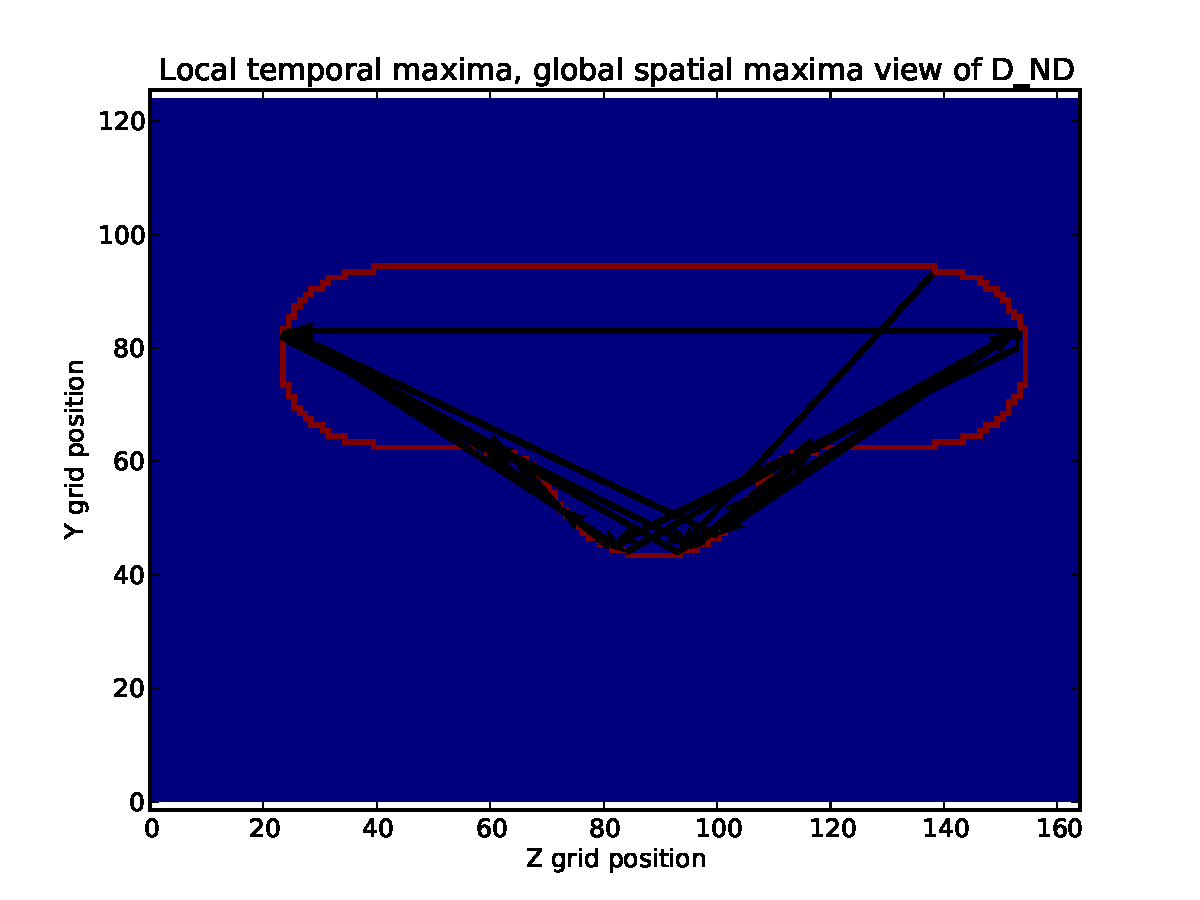
\includegraphics[width=\columnwidth]{../data/shape-randst/plots/arrow-plot-D_ND-randst-25-800-600-9700-1500}
  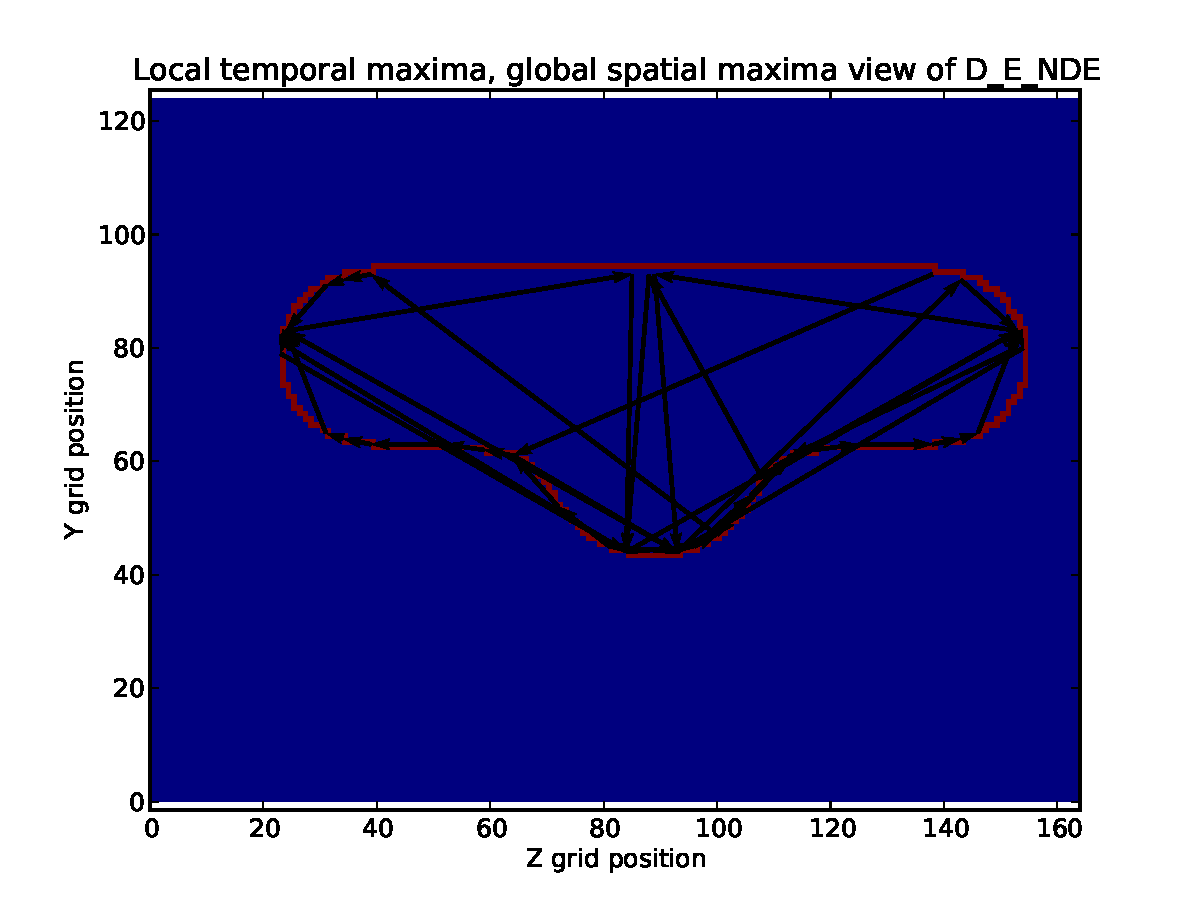
\includegraphics[width=\columnwidth]{../data/shape-randst/plots/arrow-plot-D_E_NDE-randst-25-800-600-9700-1500}
  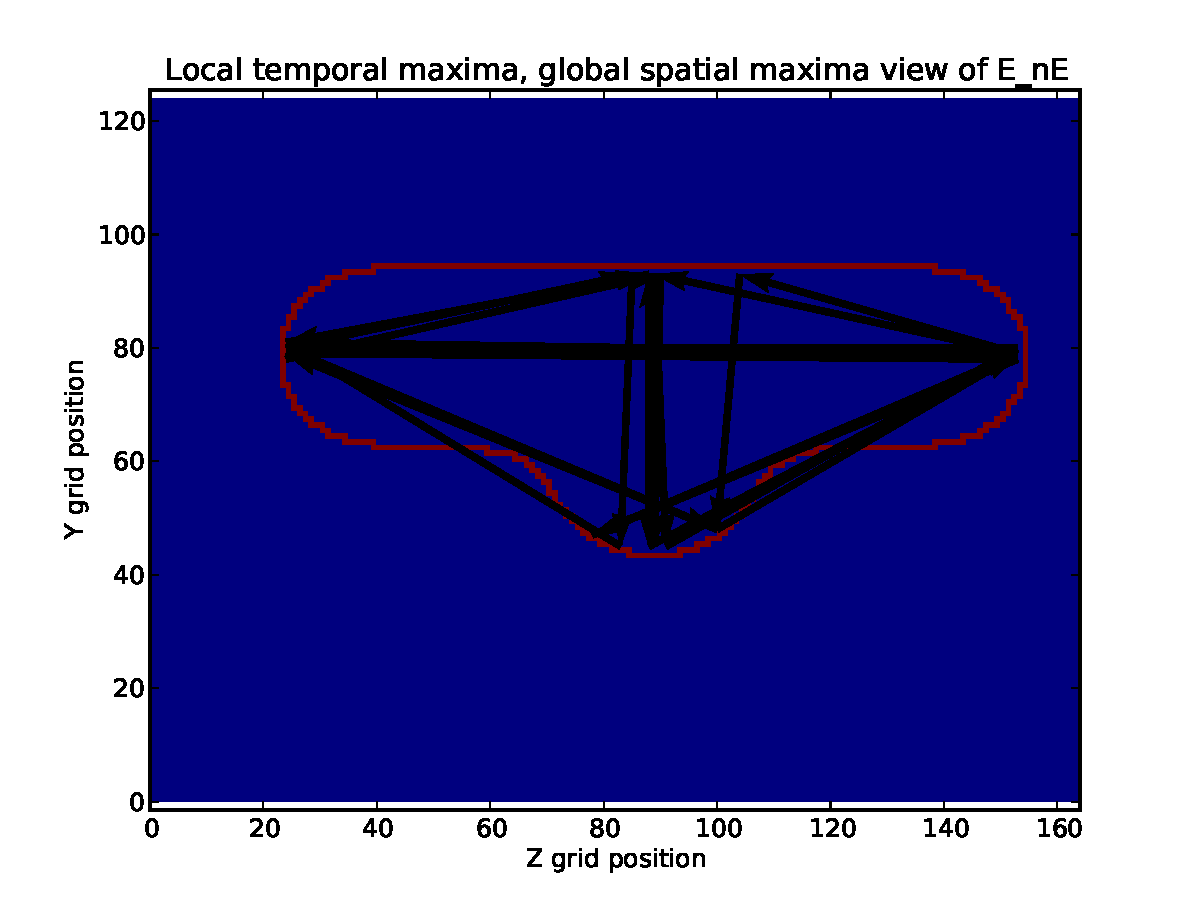
\includegraphics[width=\columnwidth]{../data/shape-randst/plots/arrow-plot-E_nE-randst-25-800-600-9700-1500}
  \caption{Arrows that connect maxima that are global in space and
    local in time. The arrow heads touch spatial, time maxima and are
    adjecent to the tails of arrows that show the very next spatial,
    time maxima. The proteins shown are wall attached MinD-ATP (top),
    wall attached MinD-MinE-ATP (middle), and cytoplasmic MinE (bottom).}
  \label{arrow-plot-randst-97-plot}
\end{figure}

Figure \ref{arrow-plot-randst-97-plot} shows three arrow plots for
this shape of cell.  It's interesting that wall attached MinD never
have global maxima in the middle flat region of the cell while both
forms of MinE, the cytoplasmic MinE and the wall attached
MinD-MinE-ATP, have a number of maxima in this region of the cell.  It
seems that the MinE never stray far from the middle of the cell - they
approach the ends and react with the other proteins, sticking for a
while on the walls.  In order for a cytoplasmic MinE to reach the very
end, it must pass a large amount of opportunity to react with MinD.
\fixme{I stopped writing this reasoning because I'm not sure it's
  valid.  Interesting thoug.  Look at this more.}


\subsubsection{Randst-98-C-Reminiscent of Mannik's cell}
\begin{figure}
  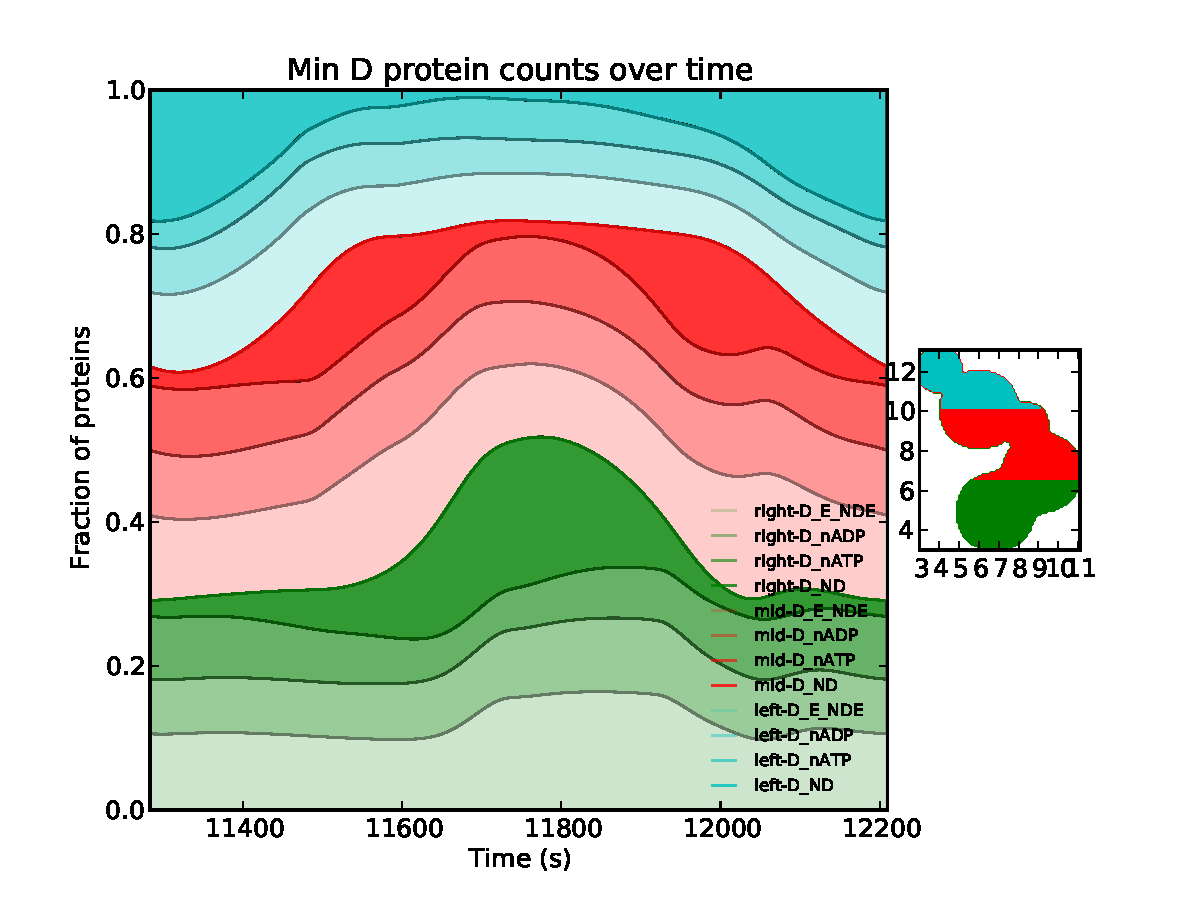
\includegraphics[width=\columnwidth]{../data/shape-randst/plots/box-plot_D--randst-25-600-800-9800-1500}
  %%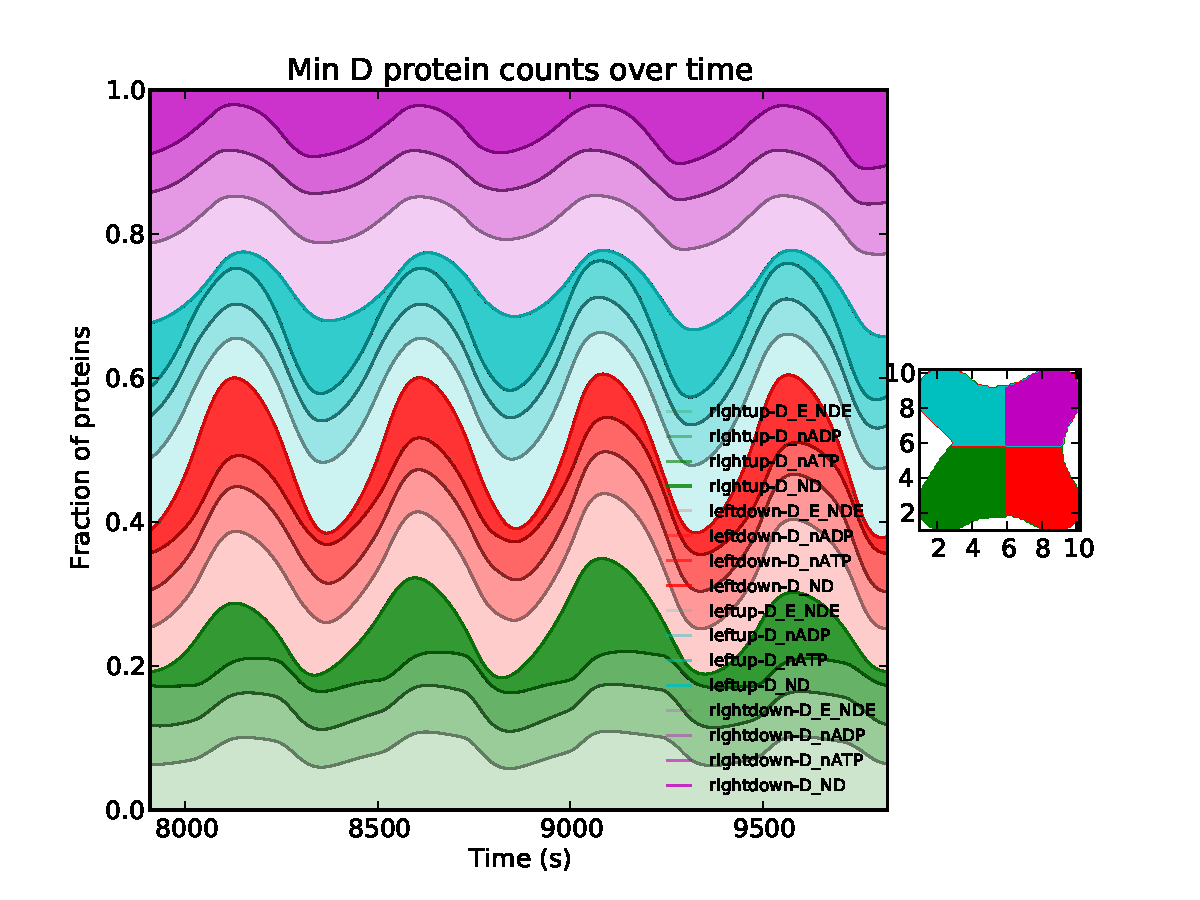
\includegraphics[width=\columnwidth]{../data/shape-randst/plots/box-plot_D--randst-25-600-600-9600-1500}
  \caption{Total protein fluctuation in the manniks squished cell
    shape.  The vertical axis shows stacked the total number of
    proteins that are of four different compound stages and in the
    different sections of the cell.}
  \label{total-oscillation-randst-98-plot}
\end{figure}

Our animations and total protein fluctuation plots (Figure
\ref{total-oscillation-randst-98-plot} for our C shape (reminiscent of
the flattened cell shown in Mannik's work) shows a very regular,
stable, simple oscillation pattern.  There are two clear ends of this
cell that oppose one another, and the protein maximum travels to one
end, where it reaches a peak, then travels through the cell to the
other end, reaching another peak, and then repeats the process.  In a
way it is similar to the simple pill shapes, in that there are two
clear endcaps and a middle section (that is in this case bends and
curves).  The protein fluctuation plots show our familiar pattern of
high spikes in wall attached MinD-ATP immediately followed by spikes
in wall attached MinD-MinE-ATP, followed by a drop in both as the
proteins move towards the other side.

\begin{figure}
  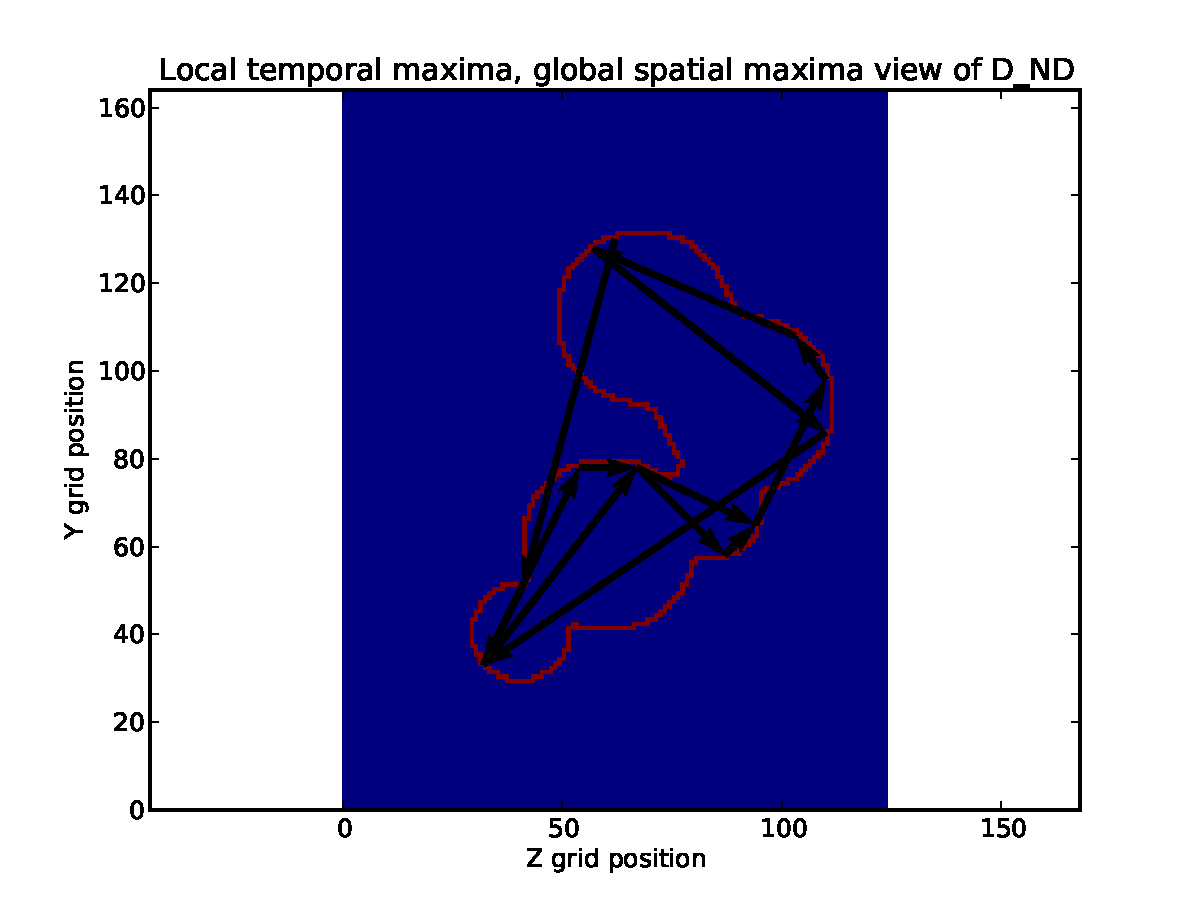
\includegraphics[width=\columnwidth]{../data/shape-randst/plots/arrow-plot-D_ND-randst-25-600-800-9800-1500}
  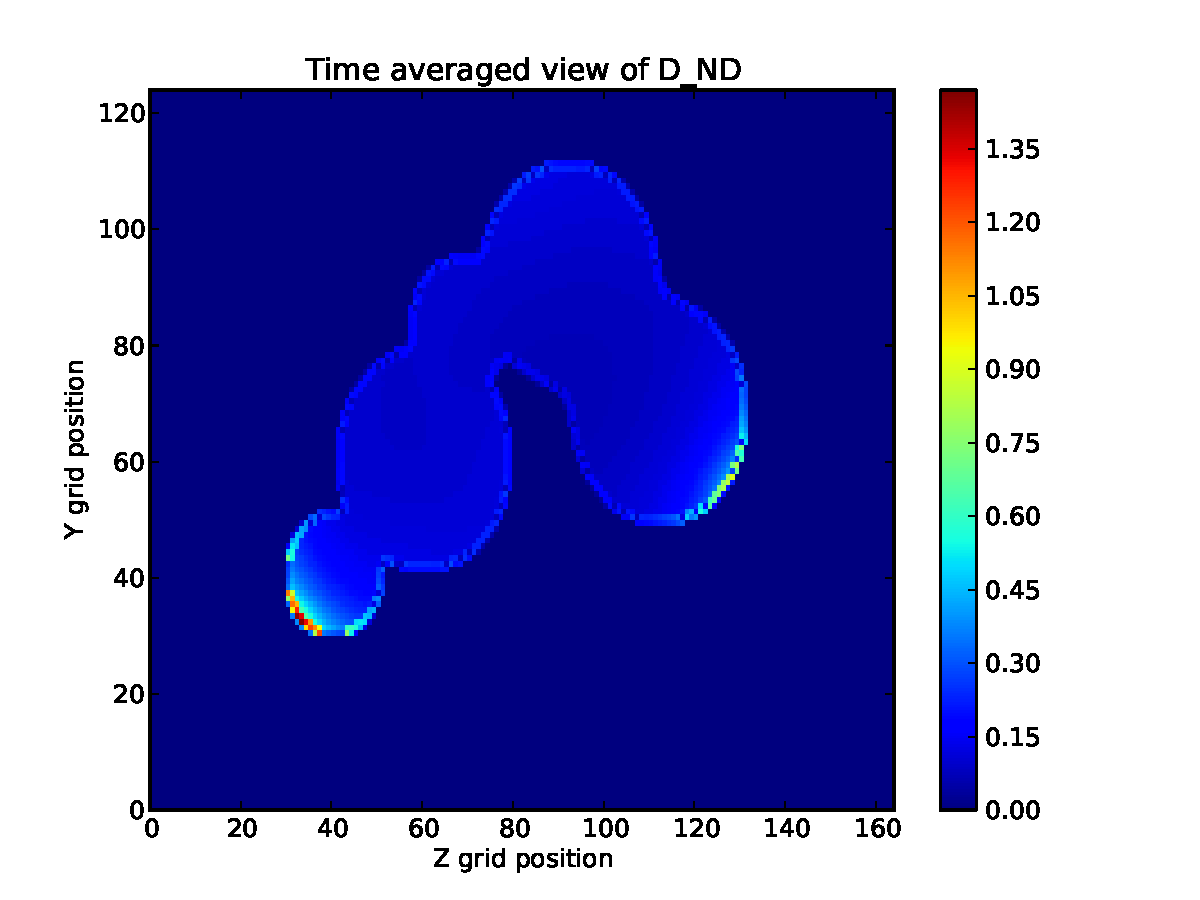
\includegraphics[width=\columnwidth]{../data/shape-randst/plots/time-map-D_ND-randst-25-600-800-9800-1500}
  \caption{(above) Arrows that connect maxima that are global in space
    and local in time. The arrow heads touch spatial, time maxima and
    are adjecent to the tails of arrows that show the very next
    spatial, time maxima. (below) An time averaged plot of the same
    proteins in the same cells shape.  The protein that is shown is
    wall attached MinD-ATP.}
  \label{arrow-plot-randst-98-plot}
\end{figure}

The arrow plot shown here is typical of mannik's squished adnormal
shape.  It shows the protein maxima moving through the cell from one
end to the other end, and back again.  The effect of this movement can
be seen in the time averaged plot directly below the arrow plot.  The
proteins spend a majority of time at the very ends of the cell.




\section{Interpretation of Data}
\section{Conclusion}
\section*{Appendix}
\bibliography{paper}











\section{Below are NOTES for the Writing}













\section{Introduction}
\fixme{I need a lot of references here!!!}
 need a lot of references here!!!  (And the writing is just
terrible) It is vital that during the process of bacterial cell
division that the cell avoid minicelling, or splitting into daughter
cells with lopsided volumes.  During this process a long FtsZ polymer
chain develops on the cell wall in the center region of the cell
acting as a guide for the cell splitting process.  in simulation that a system of Min protein interaction within
the cell will lead to a natural oscillation of the MinC protein, which
exhibits an aversion to the FtsZ polymer, from one cell end to the
other that will leave the center free of any build up of MinC.  This
will allow for the PtsZ chain to develop in the center and not at the
ends, where the two nucleiods are housed.  The interaction takes place
between MinE,MinD, and MinC, which naturally associates with MinD.

A significant amount of work has been done in simulating and studying
the dynamics of the Min protein system and cells. A number of
different models have been simulated and studied.  They divide into
two natural groups - stochastic (specific protein positions are
tracked at all times) and deterministic (protein averages are used
along with rate constants to simulate interaction). They also split up
into other groups - cooperative attachement (MinD on the cytoplasm is
attracted to other MinD on cytoplasm, shown by non-linear attachement
on walls experimentally).  Huangs' 2003 and Meinhardt and De Boer 2001
are of this type.  Huang's seuccessfully predicts that breakdown of
striped oscillation pattern occurs when exchange of ATP for ADP bound
to cytosolic MinD is not too fast.  There is as well aggregation
current models, characterized by the proteins moving along the
membranes in a way so that they're attracted to other proteins on the
walls.  We are simulating Huang's model, so a further test of the
robustness of the oscillations with wild type values, and as well
compare against exprimental evidence given by mannik.  We use Huang's
becuase of the success so far, and then also the other type
(aggregation current models) depend on there being limited binding
spots on the membrane for minD.  This author also states that the
deterministic models have largely varified stochastic model
results.\cite{kruse2007experimentalist}

It has also been observed that the spatial characteristics of
oscillation is not effected by broad ranges of tempurature changes
(although the frequency does vary) allowing for very robust cell
division that is not dettered by environmental tempurature
fluctuations. \cite{touhami2006temperature}

We wish to subject Huang's seminal model to more harsh geometrical
tests of robustness and compare results to the new experimental
results of Mannik.\fixme{this link doesn't work = cite{mannik2012robustness}}

Models also introduce the affect of cardiolipin, an anionic
phospholipid that collects on regions of high negative curvature (the
membrane of the cell poles) and attracs MinD, since it had been
observed that minD binds preferetntially in regions enriched with
these phospholipids \cite{drew2005polymerization}\cite{cytrynbaum2007multistranded}. However, this
mechanism of combined clustering, phospholipids and MinD has not been
observed in real cells.  \cite{halatek2012highly}

A mathematical model that describes the building of the FtZ polymer
along the midsection cell membrane.  Solved numerically using a finite
volume method. \cite{zhang2013mathematical}

Variations of the Huang 2003 model that attempt to more accurately
account for the details of molecular interaction, focusing on the
mechanism of MinD binding to other MinD on the cell membrane.  These
models confirm the major results obtained by Huang's model, while
showing some interesting additional features.
.\cite{drew2005polymerization}\cite{fange2006noise}\fixme{this last
  reference sounds like maybe the stochastic changes they made to the
  model cause the simulations to be more accurate in certain, odd
  cases.  Should we have used this model?}

More general biochemical models have also been used to study the MinD
system and show consistent results.\cite{arjunan2010new}

Stochastic models that area based on Huangs mean-field model but take
chemical fluctuations into account in a discrete fashion show the same
results as Huang's simulations in ordinary cell shapes, and better
predict experimentally observed oscillations in round cell
shapes.\cite{fange2006noise}

Purely theoretical models have been constructed that rely on min
protein's mobility on the membranes and tendency to cluster
together.\cite{kruse2002dynamic}\cite{howard2005cellular} \fixme{read
  and write about these}

Huang has also made simulation studies of round cell shapes and shown
that oscillations occur in these cell shapes, and that their behavior
depends on the radius of the shape. They show that the Min proteins can
select the long axis of the nearly round shapes based soley on the
geometry of the cell.\cite{huang2004min} \fixme{definately want to get
  this paper and read it}

Previous experimental studies have shown that MinC, known to inhibit
the FtZ polymer, exhibits an oscilatory, pole to pole behavoir in conjunction with
MinD and MinE. \cite{hu1999topological}

The function of the Min system might not be restricted to proper cell
division.  There is evidence that it is instrumental in the
dissasembly of the cytokinetic ring directly after cell division,
insuring that cell division takes place only once per cell
cycle. \cite{van2010mincdj}

Other simulations have been shown to exhibit oscillations in the
cylinder shaped cell.  While Huangs' 2003 study involves stages of
protein compounds (attached proteins), the differential equations
governing protein mobility in this study are designed with free
unattached proteins who interact with eachother.  Huang does cite this
paper so we can say that he followed and improved upon these
simulations.\cite{meinhardt2001pattern}

The MinE has been observed in the center of the cell and it's ability
to counteract what's refered to as MinCD cell division inhibitor has
been known.  It's been found that its not stationary but undergoes
repetitive movement back and forth. \cite{fu2001mine}

Previous studies have been made of the Min system's associtation with
the cell membrane
\cite{hsieh2010direct}\cite{mileykovskaya2003effects}. Previous
studies have shown that phospho lipids on the cell wall attract
MinD/MinE proteins and reduce ATPase activity.  It's further been
shown that the proteins interact preferebly with anionic lipids that
are localized at the poles of the cell.\cite{renner2012mind}


Expreiemntal studies have been made of the process of septum formation
in the middle of the pill shaped cell and its effect on MinD
oscillations, leading to the conclusion that it is geometry of septum
formation that allows for the creation of two MinD oscillation systems, one
in each daughter cell. \cite{juarez2010changes}

It is vital that the process of bacterial cell division result in a single
nucleiod in each daughter cell.  The cell must avoid minicelling, or
splitting into daughter cells with lopsided volumes.  One of the mechanisms
the cell employs in order to avoid this is to allow a long FtsZ polymer
chain to develop on the cell wall in the center of the cell.  This chain
acts as a guide for the cell splitting process.  Huang et all have shown in
simulation that a system of Min protein interaction within the cell will
lead to a natural oscillation of the MinC protein, which exhibits an
aversion to the FtsZ polymer, from one cell end to the other that will
leave the center free of any build up of MinC.  This will allow for the
PtsZ chain to develop in the center and not at the ends, where the two
nucleiods are housed.  The interaction takes place between MinE,MinD, and
MinC, which naturally associates with MinD.

Mannik et all have shown that the formation of irregular cell shapes
adversly effects the Min system's ability to maintain their regular
oscillatory behavior (cramming into spaces).

\subsection{What is the MinD system and why is it important?}


-Systm of proteins in E.Coli and other cells.
-Theorized to be instrumental in cell citokenisis. Reference experiments
\subsection{How proteins move in cell}
-Reference experimental showing proteins oscillating
-Reference theory showing difEQ model shows oscillations
-Reference Mannik shoving into crevices.
-Worthwhile studying effect of walls shape on the movement of cells
(Sign post of what to expect from this paper)

\section{Methods and Initial Conditions}
\subsection{Mathematical Model} %shouldn't be a scripty mu
The model for the behavior of the MinD and MinE proteins inside the cell
implemented the same set of 5 reaction-diffusion equations described in the paper
by Huang et al (equations 1, 2, 3, 4, and 5). A 3d grid was constructed in
cartesian coordinates with a grid spacing of .05 $\mu$m. From there, we
were able to define a cell shape on the grid, and solve the
reaction-diffusion equations numerically to observe the time evolution of
the MinD and MinE concentrations inside the cell.

Our simulation used the same diffusion constants and reaction rates as
Huang et al, which are

\begin{gather*} %format better
  \mathcal{D}_D = \mathcal{D}_{E}  = 2.5 \mu \textrm{m$^2$ / sec}, \\
  \sigma_D^{\textrm{ADP $\rightarrow$ ATP}}  = 1/\textrm{sec},  \sigma_D = 0.025 \mu \textrm{m/sec}, \\
  \sigma_{dD}  = 0.0015 \mu \textrm{m$^3$/sec}, \\
  \sigma_{de}  = 0.7/\textrm{sec}, \sigma_E = 0.093 \mu \textrm{m$^3$/sec}.
\end{gather*}

To test our computational model, we implemented a pill shaped cell, and
tested using the same cell parameters as Huang et al, which were a radius
of 0.5 $\mu$m in the middle and at the spherical endcaps, and two different
cell lengths of 4 $\mu$m and 10 $\mu$m. We found the same type of
oscillations as in their paper using these initial conditions, verifying
that our model works as intended. Below are snapshots of MinD and MinE
concentrations at 5 second timestamps in the 4 $\mu$m cell:
\newline
\newline
[insert 5 second time stamps of 4 $\mu$m sim]
\newline
\newline
We then began to define other, non-traditional cell shapes for the purpose of
modeling squished and perturbed E. coli cells, which were created
experimentally in Mannick et al. To achieve this, we went with a
cartesian lattice rather than the cylindrical lattice used in Huang et
al's simulations, as it allows for more flexibility in defining the
cell shape. Some of the cell shape models included a flattened pill
(stadium shape), an ellipsoid, a spherical cell, and various randomly
generated smooth shapes, such as those in the figures below.
\newline
\newline
[insert memf print of 2-3 cell shapes]
\newline
\newline
To interpret the results, we generated several different plot views of
the printed simulation data. These plots included a time averaged view
of the protein densities in the cell; a plot tracking the location of
protein concentrations that were global maxima in space and local maxima in
time; and an animated view that showed the actual dispersion of
protein concentrations in the cell over time.
\section{Specific Results}
%-Datahjhuj and plots that show concrete results. Pill normal is for the establishing that we have what works, reference  other paper, then modify, is the idea.
\section{Pill Shape}
\fixme{Be more exact about what exactly Nd is versus nATP, in terms of
  the unit and dimensions.  The plotting may need to be changed}
Figure %%\ref{frequency-plot-40-20-0-0-150} shows the protein density
fluctuations at a point in space adjecent to a polar wall.  At each
collection of peaks the proteins reach their zenith in an order that
agrees with the qualitative picture described by
Huang\cite{huang2003dynamic}, except for nADP peak.  The peaks start
with a maxima of ATP-MinD accumulating at the walls \fixme{Need a
  better way to refer to compounds}. This peak is followed by a peak
in Nde, or ATP-MinD-MinE, as the cell is converted on the wall from
the former to the latter compound.  As this compound splits apart and
leaves the wall we see a peak in nE, or MinE in the cytoplasm.  This
is then followed by a broader peak in nATP, or the MinD-ATP compound,
as minD-ADP is (changed but I forgot the name for it) into minD-ATP in
the cytoplasm.  The minD-ATP naturally diffuses away from the pole,
which is shown by the broad nature of this peak.  All of these peaks
fit the qualitative picture except for the sharp MinD-ADP peak.  One
could except that it is a sharp peak, meaning that the MinD-ADP proteins
do not last in the cytoplasm for very long before they are converted
(once again forgot the name) into MinD-ATP.  The location of the peak
in the time dimension is troubling, however, since that we would
expect it to occur just after the peak in Nde, since the wall-bound
MinD-ATP-MinE proteins are the ones that split up and leave the wall,
creating both the MinE and the MinD-ADP.  One would expect to see the
minD-ADP peak to coincide in time with the minE peak, but it instead
coincides with the wall-bound MinD-ATP-MinE peak. (Although you can
maybe sort of convince yourself otherwiase, really looking at it).

%% \begin{figure}
%%   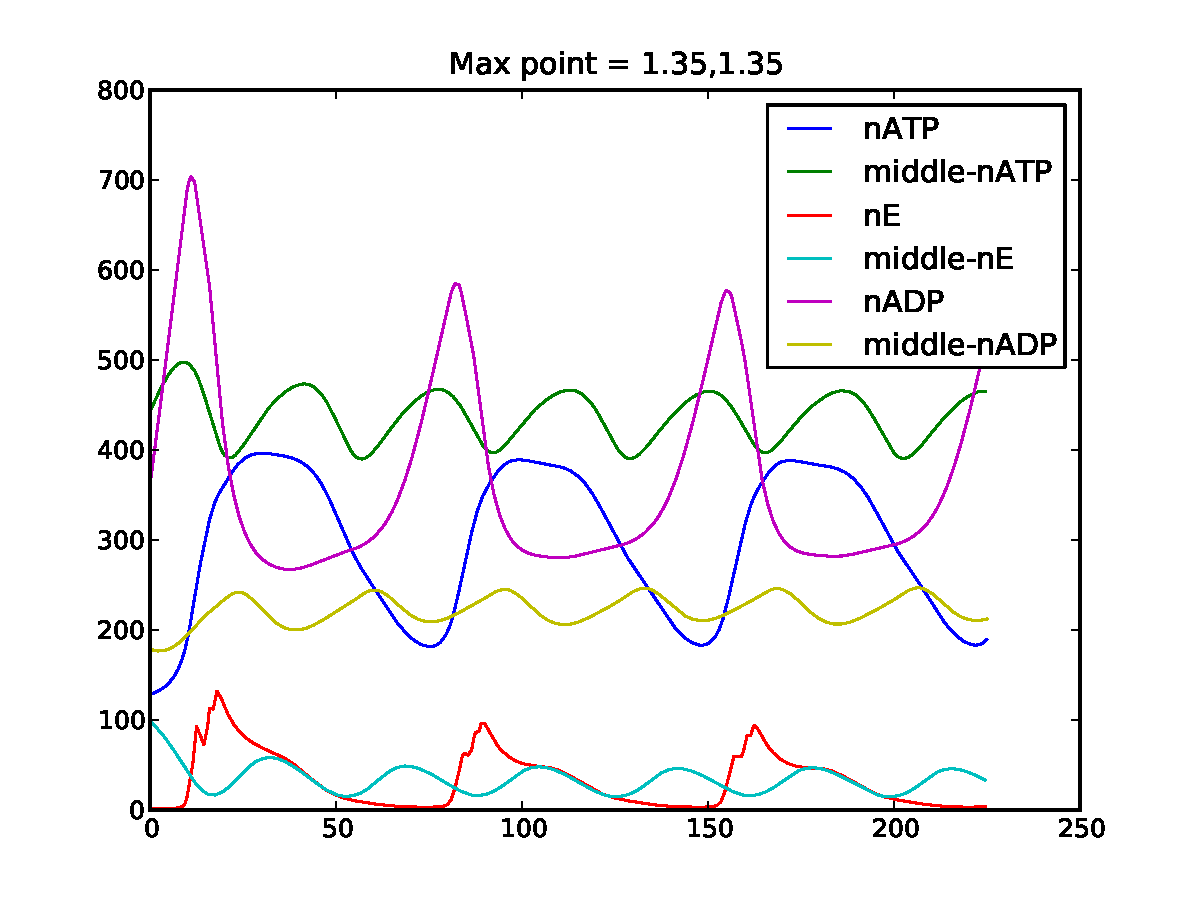
\includegraphics[width=\columnwidth]{../data/shape-p/plots/frequency_plot_all_middle-p-40-20-0-0-150.pdf}
%%   \caption{A comparison of protein density fluctuation with time
%%     against the polar wall and at a point in the center of the
%%     z-length and adjacent to the wall, in the cytoplasm.  The cell is
%%     pill shaped and has dimensions of 4$\mu m$ by 2$\mu m$.  }
%%   \label{frequency-plot-40-20-0-0-150}
%% \end{figure}

The theory states that the aversion of the FtsZ polymer to the MinC
protein is responsible for the FtsZ polymer setting up in the center
of the cell as opposed to at the cellular poles.  The MinC protein in
turn natrually associates with the minD protein that is modelled in
Huang's differential equations.  \fixme{look this up and write this
  again} The theory is dependent on there being a significant
difference in protein density between the center and polar regions. It
is worthwhile examining this difference in detail.  Figure
%%\ref{frequency-plot-40-20-0-0-150} shows a comparison of density
fluctuation over time at a point adjacent to the polar cell wall and
at a point adjacent to the cell wall in the center region of the cell.
The different proteins show different relationships between their
maxima and minima.  The MinD-ADP show sharp spikes at the poles and
much smaller oscillations at in the middle.  The values at the poles
are always greater than those in the middle, and the polar peaks
exhibit densities that are roughly 2.5 times greater than the maxima
in the center (\fixme{this factor and the following factors will be put
  into a table of comparisons for each protein and for the different
  cell sizes}).  The MinD-ATP densities show a very different trend.
For these it is the center density that is almost always greater than
the polar density.  The difference in density at the pole versus the
middle is a factor of roughly .85 (once again we'll do this more
officially in a table).  The MinE is similar to the MinD-ADP
comparison.  It shows a difference in maxima by a factor of roughly 2.
The MinC protein is associated with the minD protein, so perhaps the
most important camparison is between the nfl-MinD (MinD protein in all
its forms) at the ends and in the center of the pill.  This shows
sharp spikes at the pills and a maxima difference factor of roughly
1.25. \fixme{I'd like to analyze further what this means for the FtZ
  polymer.  Would a difference like this really have a big effect?
  What sort of effect should it have, looking at experimental data?
  One thing is that Mannik (is it Mannik?) genetically deletes the
  MinC protein and they get 73 percent proper cell division.  It
  really would be good to do a more extensive analysis here,
  referencing what other papers say about this.}

It would be good here to add the time map plots and discuss the idea
about the proteins spending most of their time in the center of the
cell.

Figure also shows that the middle
density oscillates at a frequency that is twice that of the polar
regions, which is to be expected considering the symmetry of the
center compared to the that of the polar regions.  Also, the
difference between density maxima and minima each oscillation is
smaller for the middle points than for the polar points.  This is
evident from simply watching the simulation movies - the fluctulations
are more extreme in the polar regions.

Add a table here that shows the period of oscillations versus the cell
dimensions.  Do the mathematical solution of the differential
equations for an infinite long cylinder with different widths to see
how fast the mxima move and compare (Dr. Roundy says that making the
radial speed infinite would help.


Pill Normal section -
Our goal with this project was to test whether or not the computational
model developed by Huang et al was consistent with the newer experimental
results (squishing E Coli) produced by Mannick et al. We generally see
that:

- Protein concentrations bounce around to areas with high curvature.
- - example: nflD randst 1 6 6 99 tri-polar zones with tri-polar concentrations
- - nflE the same
- There is some time delay between where different protein types appear.



The pills with larger cylindrical widths, 4.00 3.00 (the wider pill shapes)
exhibit oscillations with maxima reached on either side (half period
times) 30s, 70s, 110s, so first half oscillation occured in 30s, the
next two in 40s

The 4.00 2.00 pills exhibit a similar pattern, but max out at times
25s,55s,85s,115s, so thirty seconds each half period.  Seemed once again that
the first oscillation had a higher max density, then settled down.  I
wonder if extremely increasing the starting condition density
lopsidedness will still yield a settle down pattern with the same max
densities?  Is this dependent on shape/size?

The 4.00 0.50 pill seemed to show oscillations of 20 second half
periods very consistently.  Density maximum did not seem to lose
intensity.  Seemed to be the same each oscillation.

 Also with this, when look at the periods and max
denisty/min density ratio, consider the size dimensions of the pill
shape and see if can see a mathematical relation.

The nflE 4.00 0.50 shows a very large difference in center highest density
versus pole highest density (during a maxima).  Is this perhaps the
protein that's more important.

Looking at the extrema plots - one very interesting thing is the 4.00
2.00 ATP extrema, which shows the extrema only in the center of the
cell.  The other proteins for this shape show the extrema to be at the
ends.  Also, it seems the 4.00 3.00 cell shapes for these plots are
missing.  Very interesting to see if there is a certain protein that
has its maxima in the center of the cell, while the others have maxima
elsewhere.  Tells a story that could maybe relate to the other shapes.

Also, try starting the cells with density only in the corner.  Now the
extrema go down the center of the cell, see if there would remain a
lopsided nature of the oscillations if you started it like this instead.

The very long cells have very long periods

The time map plots seem inconsistent in that some show the highest
densities on the poles, some in the centers, some on just one pole.
For these want to run starting from a time when the proteins are
evenly spread out (so between two maxima) and stop at a similar pointe
at the end.

The time map plots that I believe though sometimes show that the max
density time-wise is actually in the middle of the cell!  Make sure we
have a good, longer view of this being true.


Important


Pill Short -
     -Know how short is too short

Randst 99 -

\section{Randst shape}
whats the difference between the extremes in density at different
places (like the density max at the poles and at the rims in the
center).  Still need to do this.

There are sudden bursts in the nflE protein plots, at the poles. Their
density maxima build very quickly then diffuse more slowly.

\subsection{randst-96}
The star shape (randst-96) Shows oscillations in nflD horizontally,
two poles to two poles.  There is sometimes a small amount of lag
between the upper maxima moving horizontally and the lower.  Half
periods take roughly 25s. Dimensions are roughly 5.00 by 5.00?  Check
this.  The nflE short bursts do develop lag between when the top and
the bottom go off.  Should coordinate this with the nflD lag.

Tried to see if there is a time correlation between nflE and nflD but
the maxima seem to appear in the poles at roughly the same time.

Watched Nd and nE simulations next to each other at same time.  Both
have maxima that build up right at the walls (in the corners) and then
subside.  It's clear that the nE density bursts appear directly after
the Nd bursts.  The Nd bursts are subsiding as the nE bursts are
rising up.  The Nd reaches a time maxima just before the nE.  This is
true in each corner, so that when the maxima are lopsided top to
bottom - when the top right corner maximizes first, say, the interplay
between nE and Nd remains very clear in those corners where and when
maxima occur.

Watched nATP and nADP together.  nATP maxima seem to follow slightly
after nADP maxima.  This is not surprising since in rotation nATP
follows after nADP.  nATP maxima is more spread out - inbetween pole
maxima there is more spread out maxima in the center.  This should
show itself in the time map plotting.  About this - the percentage
difference seem to be the same between the non-max places and max
places, roughly, its just that the nATP seems to have a max region
that covers a wider area throughout the oscillation (or at least in
between the maxima points in the oscillation).

Also watched the Nd next to the nATP.  The Nd maximize more extreme in
the corners up against the walls.  The nATP density follows the Nd
maxima, it looks like the nATP maxima follows the Nd.  So if the Nd
appears somewhere (in a corner) then the nATP will travel there to
follow.


\subsection{randst-97}
Randst 97 nflE starts with small maxima, not much difference at all,
then actually builds to high maxima at the poles.
\subsection{randst-99}
Randst 99 (sort of triangle) is roughly dimensions of 3.5 by 3.5?
nflD oscillations appear to be half periods of 25s as well.  Maxima appear
at the poles and in the interim there are weak maxima in center pole.
\subsection{randst-98}
Funny randst shape 98 shows nflD oscillations of about 30s or so.

nADP and nATP side by side.  nADP maximizes in the corners right
before the nATP maxima follows.  Makes sense looking at equations.
Once again the nATP maxima is more spread out, where maxima in nADP
appear more just at walls.

Nd and nATP side by side.  Nd maximizes at walls and the nATP moves in
to follow it

Nd and nE side by side.  Nd maximizes in corners and then the nE also
maximizes in the corners.  The nE maxima appear in these sort of quick
bursts in the corners, along with a slower broader movements away from
that corner after the burst and into the next, where another sharp
burst occurs.  The Nd bursts occurs after the Nd as subsided in that
corner, and really by the time the burst maximizes, the Nd is already
on its way over and starting to build on the otehr side.

Randst nflD doesn't show much oscillation at all, but we start it so
that the density is not max at the pole.






%%\begin{figure}
%%   \includegraphics[width=\columnwidth]{../data/shape-randst/plots/time-map-compare-randst-10-80-60-980-150.pdf}
%%   \caption{randst 98}
%%   %\label{fig:pair-distribution-3}
%% \end{figure}
%% \begin{figure}
%%   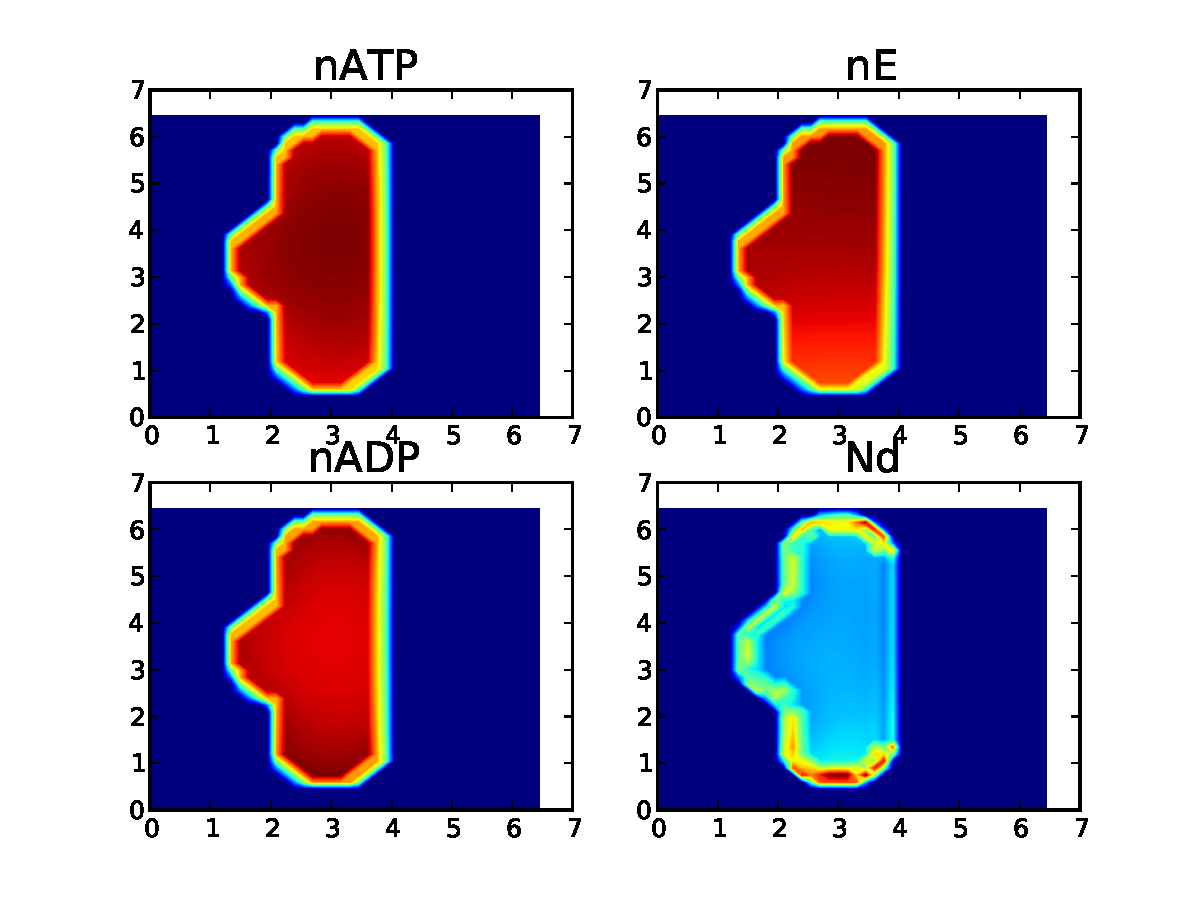
\includegraphics[width=\columnwidth]{../data/shape-randst/plots/time-map-compare-randst-10-60-60-970-150.pdf}
%%   \caption{randst 97}
%%   %\label{fig:pair-distribution-3}
%% \end{figure}
%% \begin{figure}
%%   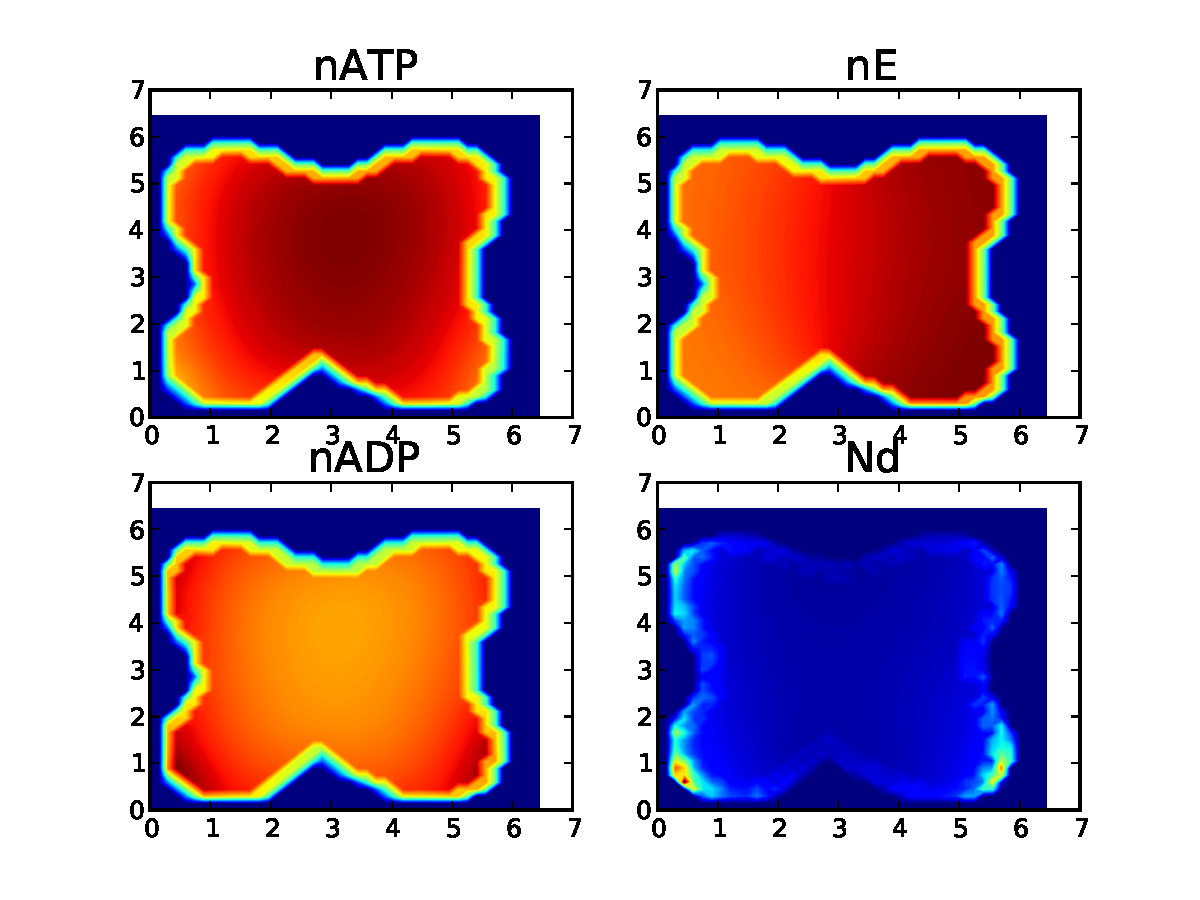
\includegraphics[width=\columnwidth]{../data/shape-randst/plots/time-map-compare-randst-10-60-60-960-150.pdf}
%%   \caption{randst 96}
%%   %\label{fig:pair-distribution-3}
%% \end{figure}

Randst 98 -

Randst 97 -

Randst 96 -

Triangle -


\section{Interpretation of Data}
-Discussion of conceptual reasons of why we see what we see
-Plots that are more interpretive (area-rating)
-Some sort of predictive claim?

\section{animate?}
%%\animategraphics[height=2.8in,autoplay,controls]{12}{../data/shape-randst/plots/movie-density-Nd-96/animate_}{0}{120}



\section{Conclusion}



\end{document}
